\documentclass{article}
\usepackage[margin=2cm]{geometry}
\usepackage{amsmath}
\usepackage{amssymb}
\usepackage{amsthm}
\usepackage{amsfonts}
\usepackage[utf8]{inputenc}
\usepackage{graphicx}
\usepackage{caption}
\usepackage{listings}
\usepackage{multicol}\setlength{\columnsep}{1cm}
\setlength{\parindent}{0pt}

\usepackage{enumitem}
\setlist{nosep}
\setlistdepth{9}
\setlist[enumerate,1]{label=$\arabic*.$}
\setlist[enumerate,2]{label=$\alph*.$}
\setlist[enumerate,3]{label=$\roman*.$}
\setlist[enumerate,4]{label=$(\arabic*)$}
\setlist[enumerate,5]{label=$(\alph*)$}
\setlist[enumerate,6]{label=$(\roman*)$}
\setlist[enumerate,7]{label=$\arabic*$}
\setlist[enumerate,8]{label=$\alph*$}
\setlist[enumerate,9]{label=$\roman*$}
\renewlist{enumerate}{enumerate}{9}

\newcommand{\Xset}{\!\leftarrow\!}
\newcommand{\Xund}{\rule{.4em}{.4pt}} % underscore
\newcommand{\Xin}{\!\in\!}
\newcommand{\Xeq}{\!=\!}
\newcommand{\Xlb}{[\![}
\newcommand{\Xrb}{]\!]}
\newcommand{\Xmap}{\!\mapsto\!}
\newcommand{\XB}{\mathcal{B}}
\newcommand{\XD}{\mathcal{D}}
\newcommand{\XF}{\mathcal{F}}
\newcommand{\XI}{\mathcal{I}}
\newcommand{\XL}{\mathcal{L}}
\newcommand{\XN}{\mathcal{N}}
\newcommand{\XO}{\mathcal{O}}
\newcommand{\XP}{\mathcal{P}}
\newcommand{\XS}{\mathcal{S}}
\newcommand{\XT}{\mathcal{T}}
\newcommand{\XX}{\mathcal{X}}
\newcommand{\YB}{\mathbb{B}}
\newcommand{\YF}{\mathbb{F}}
\newcommand{\YN}{\mathbb{N}}
\newcommand{\YT}{\mathbb{T}}
\newcommand{\YQ}{\mathbb{Q}}

\newcommand{\Xstirling}[2]{\genfrac{\{}{\}}{0pt}{}{#1}{#2}}

\makeatletter
\newcommand*{\Relbarfill@}{\arrowfill@\Relbar\Relbar\Relbar}
\newcommand*{\Xlongeq}[2][]{\ext@arrow 0055\Relbarfill@{#1}{\text{#2}}}
\newcommand*{\Xbar}[1]{\overline{#1\vphantom{\bar{#1}}}}
\makeatother

\theoremstyle{definition}
\newtheorem{Xdef}{Definition}
\newtheorem{XThe}{Theorem}
\newtheorem{XLem}{Lemma}

\title{Tagged Deterministic Finite Automata with Lookahead}
\author{Ulya Trofimivich}
\date{March 2017}

\begin{document}

\maketitle

\begin{abstract}
\noindent
This paper extends the work of Laurikari [Lau00] [Lau01] and Kuklewicz [Kuk??] on tagged deterministic finite automata (TDFA)
in connection with submatch extraction in regular expressions.
I augment TDFA with 1-symbol lookahead, which results in significant reduction of tag variables and operations.
Lookahead-aware automata may have slightly more states, but they are more amenable to optimizations and as a rule result in both smaller and faster code.
The proposed algorithm can handle repeated submatch and therefore is applicable to full parsing.
Furthermore, I consider two disambiguation policies: leftmost greedy and POSIX.
I formalize the algorithm suggested by Kuklewicz
and show that Kuklewicz TDFA have no overhead compared to Laurikari TDFA or automata that use leftmost greedy disambiguation.
All discussed models and algorithms are implemented in the open source lexer generator RE2C.
\end{abstract}
%\vspace{1em}

\begin{multicols}{2}

\section*{Introduction}

RE2C [Bum94] [web??] is a lexer generator for C: it compiles regular expressions into code.
Unlike regular expression libraries such as TRE [Lau01] or RE2 [Cox??], RE2C has no restriction on preprocessing time
and concentrates fully on the quality of generated code.
RE2C takes pride in generating fast lexers: at least as fast as reasonably optimized lexers coded by hand.
This is not an easy goal; hand-written code is specialized for a particular environment, while autogenerated code must fit anywhere.
RE2C has a highly configurable interface and quite a few optimizations ranging from
high-level program transformations to low-level tweaks of conditional jumps.
In such setting it is undesirable to add extensions that affect performance.
\\ \\
One useful extension of regular expressions is submatch extraction and parsing.
Many authors studied this subject and developed algorithms suitable for their particular settings and problem domains.
Their approaches differ in many respects:
the specific subtype of problem (full parsing, submatch extracton with or without history of repetitions);
the underlying formalizm (backtracking,
nondeterministic automata, deterministic automata, 
multiple automata, lazy determinization);
the number of passes over the input (streaming, multi-pass);
space consumption with respect to input length (constant, proportional);
treatment of ambiguity (unhandled, manual disambiguation, default disambiguation policy, all possible parse trees).
%Their approaches differ in many respects:
%the specific subtype of problem (full parsing, submatch extracton with or without history of repeated submatches);
%the underlying formalizm (backtracking,
%nondeterministic automaton [ThoBra] [Cox],
%deterministic automaton [Ragel] [Lau00] [Gra15],
%multiple deterministic automata [SohTho],
%lazy determinization [Kuk] [Kar]);
%the number of passes over the input (streaming, multi-pass);
%space consumption (constant, proportional to the size of output [Gra] [ThoBra], proportional to length of input [Kea] [DubFee]);
%treatment of ambiguity (forbidden, manual disambiguation [Ragel], default policy [FriCar] [Gra], multiple options [ThoBra]).
Most of the algorithms are unsuitable for RE2C: either insufficienty generic (cannot handle ambiguity),
or too heavyweight (incur too much overhead on regular expressions with only a few submatches or no submatches at all).
Laurikari algorithm is special in this respect.
It is based on a single deterministic automaton, runs in one pass and linear time,
and the consumed space does not depend on the input length.
What is most important, the overhead on submatch extraction depends on the detalization of submatch:
on regular expressions without submatches Laurikari automaton shrinks to a simple DFA.
\\ \\
From RE2C point of view this is close enough to hand-written code:
you only pay for what you need, like a reasonable programmer would do.
However, a closer look at Laurikari automata reveals that
they behave like a very strange programmer who is unable to think even one step ahead.
Take, for example, regular expression \texttt{a*b*}
and suppose that we must find the boundary between \texttt{a} and \texttt{b} in the input string.
The programmer would probably match all \texttt{a}, then save the input position, then match all \texttt{b}:

\begin{small}
\begin{verbatim}
    while (*s++ == 'a') ;
    p = s;
    while (*s++ == 'b') ;
\end{verbatim}
\end{small}

And this is how the automaton would do:

\begin{small}
\begin{verbatim}
    p = s;
    while (*s++ == 'a') p = s;
    while (*s++ == 'b') ;
\end{verbatim}
\end{small}

This behaviour is correct (it yields the same result), but strangely inefficient:
it repeatedly saves input position after every \texttt{a},
while for the programmer it is obvious that there is nothing to save until the first non-\texttt{a}.
One might object that the compiler would optimize out the difference,
and it probably would in simple cases like this.
However, the flaw is common to all Laurikari automata:
they ignore lookahead when recording submatches.
But they don't have to; with a minor fix we can teach them
to delay recording until the right lookahead symbol shows up.
This minor fix is my first contribution.
\\

Another problem that needs attention is disambiguation.
The original paper [Lau01] claims to have POSIX semantics, but it was proved to be wrong [LTU].
Since then Kuklewicz suggested a fix of Laurikari algorithm that does have POSIX semantics [Regex-TDFA], but he never formalized it.
The informal description [regex-wiki] is somewhat misleading as it suggests that Kuklewicz automata
require additional run-time operations to keep track of submatch history and hence are less efficient than Laurikari automata.
That is not true, as we shall see: all the added complexity is related to determinization,
while the resulting automata are just the same (except they have POSIX semantics).
Kuklewicz did not emphasize this, probably because his implementation constructs TDFA lazily at run-time.
I formalize Kuklewicz algorithm; this is my second contibution.
\\

Finally, theory is no good without practice.
Even lookahead-aware automata contain a lot of redundant operations,
which can be dramatically reduced by the most basic optimizations like liveness analysis and dead code elimination.
The overall number of submatch records can be minimized using technique similar to register allocation.
I suggest another tweak of Laurikari algoritm that makes optimizations particularly easy
and show that they have crucial impact on the quality of code, even in the presence of an optimizing C compiler.
RE2C implementation of submatch extraction is the motivation and the main goal of this work.
\\

The rest of this paper is arranged as follows.
We start with theoretical foundations and gradually move towards practical algorithms.
Section \ref{section_regular_expressions} revises the basic definition of regular expressions.
In section \ref{section_tagged_extension} we extend it with tags
and define ambiguity with respect to submatch extraction.
In section \ref{section_tnfa} we convert regular expressions to nondeterministic automata
and in section \ref{section_closure} study various algorithms for closure construction.
Section \ref{section_disambiguation} is about disambiguation;
we discuss leftmost greedy and POSIX policies and the necessary properties that disambiguation policy should have in order to allow efficient submatch extraction.
Section \ref{section_determinization} is the main part of this paper: it presents determinization algorithm.
Section \ref{section_optimizations} highlihgts some practical implementation details and optimizations.
Section \ref{section_evaluation} concerns correctness testing and benchmarks.
Finally, section \ref{section_future_work} points directions for future work.

\section{Regular expressions}\label{section_regular_expressions}

Regular expressions is a notation that originates in the work of Kleene
\emph{``Representation of Events in Nerve Nets and Finite Automata''} [Kle51] [Kle56].
He used this notation to describe \emph{regular events}:
each regular event is a set of \emph{definite events},
and the class of all regular events is defined inductively
as the least class containing basic events (empty set and all unit sets)
and closed under the operations of \emph{sum}, \emph{product} and \emph{iterate}.
Kleene showed that regular events form exactly the class of events that can be represented by McCulloch-Pitts nerve nets or, equivalently, finite automata.
However, generalization of regular events to other fields of mathematics remained an open problem;
in particular, Kleene raised the question whether regular events could be reformulated
as a deductive system based on logical axioms and algebraic laws.
This question was thoroughly investigated by many authors (see [Koz91] for a historic overview)
and the formalism became known as \emph{the algebra of regular events} %$\mathcal{K} \Xeq (K, +, \cdot, *, 1, 0)$
or, more generally, the \emph{Kleene algebra}.
Several different axiomatizations of Kleene algebra were given;
in particular, Kozen gave a finitary axiomatization based on equations and equational implications and sound for all interpretations [Koz91].
We will use the usual inductive definition:
\\

    \begin{Xdef}
    \emph{Regular expressions (RE)} over finite alphabet $\Sigma$
    is a notation that is inductively defined as follows:
    \begin{enumerate}
        \medskip
        \item[] $\emptyset$, $\epsilon$ and $\alpha \Xin \Sigma$ are \emph{atomic} RE
        \item[] if $e_1$, $e_2$ are RE, then $e_1 | e_2$ is RE (\emph{sum})
        \item[] if $e_1$, $e_2$ are RE, then $e_1 e_2$ is RE (\emph{product})
        \item[] if $e$ is RE, then $e^*$ is RE (\emph{iteration})
        \medskip
    \end{enumerate}
    Iteration has precedence over product and product over sum;
    parenthesis may be used to override it.
    $\square$
    \end{Xdef}

For the most useful RE there are special shortcuts:
    \begin{align*}
        e^n     &\quad\text{for}\quad \overbrace{e \dots e}^{n} \\[-0.5em]
        e^{n,m} &\quad\text{for}\quad e^n | e^{n+1} | \dots | e^{m-1} | e^m \\[-0.5em]
        e^{n,}  &\quad\text{for}\quad e^n e^* \\[-0.5em]
        e^+     &\quad\text{for}\quad ee^* \\[-0.5em]
        e^?     &\quad\text{for}\quad e | \epsilon
    \end{align*}

Since RE are only a notation, their exact meaning depends on the particular \emph{interpretation}.
In the \emph{standard} interpretation RE denote \emph{languages}: sets of strings over the alphabet of RE.

    \begin{Xdef}
    \emph{Language} over $\Sigma$ is a subset of $\Sigma^*$,
    where $\Sigma^*$ denotes the set of all (possibly empty) strings over $\Sigma$.
    $\square$
    \end{Xdef}

    \begin{Xdef}\label{langunion}
    \emph{Union} of two languages $L_1$ and $L_2$ is
    $L_1 \cup L_2 = \{ x \mid x \Xin L_1 \vee x \Xin L_2 \}$
    $\square$
    \end{Xdef}

    \begin{Xdef}\label{langproduct}
    \emph{Product} of two languages $L_1$ and $L_2$ is
    $L_1 \cdot L_2 = \{ x_1 x_2 \mid x_1 \Xin L_1 \wedge x_2 \Xin L_2 \}$
    $\square$
    \end{Xdef}

    \begin{Xdef}\label{langiterate}
    n-th \emph{Power} of language $L$ is
    $$L^n = \begin{cases}
            \{ \epsilon \} & \text{if } n \Xeq 0 \\[-0.5em]
            L \cdot L^{n - 1} & \text{if } n\!>\!0
        \end{cases}$$
    $\square$
    \end{Xdef}

    \begin{Xdef}\label{langiterate}
    \emph{Iterate} of language $L$ is
    $L^* = \bigcup\limits_{n = 0}^\infty L^n$.
    $\square$
    \end{Xdef}

    \begin{Xdef}
    \emph{(Language interpretation of RE)} \\
    RE denotes a language over $\Sigma$:
    \begin{align*}
        \XL \Xlb \emptyset \Xrb &= \emptyset \\
        \XL \Xlb \epsilon \Xrb &= \{ \epsilon \} \\
        \XL \Xlb \alpha \Xrb &= \{\alpha\} \\
        \XL \Xlb e_1 | e_2 \Xrb &= \XL \Xlb e_1 \Xrb \cup \XL \Xlb e_2 \Xrb \\
        \XL \Xlb e_1 e_2 \Xrb &= \XL \Xlb e_1 \Xrb \cdot \XL \Xlb e_2 \Xrb \\
        \XL \Xlb e^* \Xrb &= \XL \Xlb e \Xrb ^*
    \end{align*}
    $\square$
    \end{Xdef}

Other interpretations are also possible;
one notable example is the \emph{type interpretation},
in which RE denote sets of parse trees [ThoBra10] [Gra15].
This is close to what we need for submatch extraction,
except that we are interested in partial parse structure rather than full parse trees.

    \begin{Xdef}
    Language $L$ over $\Sigma$ is \emph{regular} iff $\exists$ RE $e$ over $\Sigma$
    such that $L$ is denoted by $e$: $\XL \Xlb e \Xrb \Xeq L$.
    $\square$
    \end{Xdef}

The set $\mathcal{R}_\Sigma$ of all regular languages over alphabet $\Sigma$
together with constants $\emptyset$, $\{ \epsilon \}$ and operations $\cup$, $\cdot$ and ${}^*$
forms a Kleene algebra $\mathcal{K} \Xeq (\mathcal{R}_\Sigma, \cup, \cdot, *, \emptyset, \{ \epsilon \})$.

\section{Tagged extension}\label{section_tagged_extension}

In short, tags are position markers attached to the structure of RE.
The idea of adding such markers is not new:
many RE flavours have \emph{capturing groups}, or the \emph{lookahead} operator, or \emph{pre-} and \emph{post-context} operators;
all of them are used for submatch extraction of some sort.
Laurikari used the word \emph{tag}.
He did not define tags explicitly; rather, he defined automata with tagged transitions.
We take a slightly different appoach, inspired by [ThoBra10], [Gra15] and a number of other publications.
First, we define an extension of RE: tagged RE,
and two interpretations: \emph{S-language} that ignores tags and \emph{T-language} that respects them.
T-language has the bare minimum of information necessary for submatch extraction;
in particular, it is less expressive than \emph{parse trees} or \emph{types} that are used for RE parsing.
Then we define \emph{ambiguity} and \emph{disambiguation policy} in terms of relations between the two interpretations.
Finally, we show how T-language can be converted to the \emph{tag value functions} used by Laurikari
and argue that the latter representation is insufficient as it cannot express ambiguity in some RE.
\\

Tagged RE differ from RE in the following respects.
First, they have a new kind of atomic primitive: tags.
Second, we use generalized repetition $e^{n,m}$ (possibly $m \Xeq \infty$) as one of the three base operations instead of iteration $e^*$.
The reason for this is that
desugaring repetition into concatenation and iteration requires duplication of $e$,
and duplication may change the semantics of submatch extraction.
For example, POSIX RE \texttt{(a(b?))\{2\}} contains two submatch groups (aside from the whole RE),
but if we rewrite it as \texttt{(a(b?))(a(b?))}, the number of submatches will change to four.
Third difference is that repetition starts from one: zero or more repetitions are expressed as alternative between one or more repetitions and the empty word.
This is mostly a matter of convenience:
the case of zero iterations is special because it contains no tags, even if the subexpression itself does.

    \begin{Xdef}
    \emph{Tagged regular expressions (TRE)} over disjoint finite alphabets $\Sigma$ and $T$
    is a notation that is inductively defined as follows:
    \begin{enumerate}
        \medskip
        \item[] $\emptyset$, $\epsilon$, $\alpha \Xin \Sigma$, $t \Xin T$ are \emph{atomic} TRE
        \item[] if $e_1$, $e_2$ are TRE, then $e_1 | e_2$ is TRE (\emph{sum})
        \item[] if $e_1$, $e_2$ are TRE, then $e_1 e_2$ is TRE (\emph{product})
%        \item[] if $e$ is TRE and $1 \!\leq\! n \!\leq\! \infty$, then $e^{1,n}$ is TRE (\emph{repetition})
        \item[] if $e$ is TRE and $0 \!<\! n \!\leq\! m \!\leq\! \infty$, then $e^{n,m}$ is TRE (\emph{repetition})
        \medskip
    \end{enumerate}
    Repetition has precedence over product and product over sum;
    parenthesis may be used to override it.
    Additionally, the following shorthand notation may be used:
    \begin{align*}
%        e^n     &\quad\text{for}\quad \overbrace{e \dots e}^{n} \\[-0.5em]
%        e^{n,m} &\quad\text{for}\quad e^{n-1} e^{1,m-n} \\[-0.5em]
        e^n     &\quad\text{for}\quad e^{n,n} \\[-0.5em]
        e^{0,m} &\quad\text{for}\quad e^{1,m} | \epsilon \\[-0.5em]
        e^*     &\quad\text{for}\quad e^{1,\infty} | \epsilon \\[-0.5em]
        e^+     &\quad\text{for}\quad e^{1,\infty} \\[-0.5em]
        e^?     &\quad\text{for}\quad e | \epsilon
    \end{align*}
    $\square$
    \end{Xdef}

    \begin{Xdef}
    TRE over $\Sigma$, $T$ is \emph{well-formed} iff
    all tags in it are pairwise different
    and $T \Xeq \{ 1, \dots, |T| \}$.
    $\square$
    We will consider only well-formed TRE.
    \end{Xdef}

If we assume that tags are aliases to $\epsilon$, then every TRE over $\Sigma$, $T$ is a RE over $\Sigma$:
intuitively, this corresponds to erasing all submatch information. 
We call this \emph{S-language interpretation} (short from ``sigma'' or ``source''),
and the corresponding strings are \emph{S-strings}:

    \begin{Xdef}\label{defslang}
    \emph{(S-language interpretation of TRE)} \\
    TRE over $\Sigma$, $T$ denotes a language over $\Sigma$:
    \begin{align*}
        \XS \Xlb \emptyset \Xrb &= \emptyset \\
        \XS \Xlb \epsilon \Xrb &= \{ \epsilon \} \\
        \XS \Xlb \alpha \Xrb &= \{\alpha\} \\
        \XS \Xlb t \Xrb &= \{\epsilon\} \\
        \XS \Xlb e_1 | e_2 \Xrb &= \XS \Xlb e_1 \Xrb \cup \XS \Xlb e_2 \Xrb \\
        \XS \Xlb e_1 e_2 \Xrb &= \XS \Xlb e_1 \Xrb \cdot \XS \Xlb e_2 \Xrb \\
        \XS \Xlb e^{n,m} \Xrb &= \bigcup\limits_{i=n}^m \XS \Xlb e \Xrb ^i
    \end{align*}
    $\square$
    \end{Xdef}

On the other hand, if we interpret tags as symbols, then every TRE over $\Sigma$, $T$ is a RE over the joined alphabet $\Sigma \cup T$.
This interpretation retains submatch information; however, it misses one important detail: \emph{negative} submatches.
Negative submatches are implicitly encoded in the structure of TRE:
we can always deduce the \emph{absense} of tag from its \emph{presence} on alternative branch of TRE.
To see why this is important, consider POSIX RE \texttt{(a(b)?)*} matched against string \texttt{aba}.
The outermost capturing group matches twice at offsets \texttt{(0,2)} and \texttt{(2,3)}.
The innermost group matches only once at \texttt{(1,2)}; there is no match on the second outermost iteration.
POSIX standard demands that we report the absence of match \texttt{(?,?)}.
Even aside from POSIX, we might be interested in the whole history of submatch.
Therefore we will rewrite TRE in a form that makes negative submatches explicit
(by tracking tags on alternative branches and inserting negative tags at all join points).
Negative tags are marked with bar, and $\Xbar{T}$ denotes the set of all negative tags.

    \begin{Xdef}\label{deftlang}
    Operator $\XX$ rewrites TRE over $\Sigma$, $T$ to a TRE over $\Sigma$, $T \cup \Xbar{T}$:
    \begin{align*}
        \XX(\emptyset) &= \emptyset \\
        \XX(\epsilon) &= \epsilon \\
        \XX(\alpha) &= \alpha \\
        \XX(t) &= t \\
        \XX(e_1 | e_2)
            &=      \XX(e_1) \chi(e_2) \mid \XX(e_2) \chi(e_1) \\
            \text{where }
                &\chi(e) = \Xbar{t_1} \dots \Xbar{t_n} \text{ such that} \\
                &t_1 \dots t_n \text{ are all tags in } e \\
        \XX(e_1 e_2) &= \XX(e_1) \XX(e_2) \\
        \XX(e^{n,m}) &= \XX(e)^{n,m}
    \end{align*}
    $\square$
    \end{Xdef}

    \begin{Xdef}\label{deftlang}
    \emph{(T-language interpretation of TRE)} \\
    TRE over $\Sigma$, $T$ denotes a language over $\Sigma \cup T \cup \Xbar{T}$:
    $\XT \Xlb e \Xrb = \XL \Xlb \widetilde{e} \Xrb$, where $\widetilde{e}$ is a RE
    syntactically identical to TRE $\XX(e)$.
    $\square$
    \end{Xdef}

The language over $\Sigma \cup T \cup \Xbar{T}$ is called \emph{T-language}
(short from ``tag'' or ``target''), and its strings are called \emph{T-strings}.
For example:
\begin{align*}
    \XT \Xlb \beta &| (\alpha 1)^{0,2} \Xrb
=
    \XT \Xlb \beta \Xrb \cdot \{\Xbar{1}\} \cup
    \XT \Xlb (\alpha 1)^{1,2} | \epsilon \Xrb \cdot \{\epsilon\} = \\
&=
    \{\beta \Xbar{1}\} \cup
    \big(\XT \Xlb \alpha 1 \Xrb
            \cup \XT \Xlb \alpha 1 \Xrb \cdot \XT \Xlb \alpha 1 \Xrb
        \big) \cdot \{\epsilon\}
        \cup \{\Xbar{1}\} = \\
&=
    \{\beta \Xbar{1}\} \cup
    \{\alpha 1 \} \cup
    \{\alpha 1 \alpha 1 \} \cup
    \{\Xbar{1}\} = \\
&=
    \{\beta \Xbar{1}, \Xbar{1}, \alpha 1, \alpha 1 \alpha 1 \}
\end{align*}

    \begin{Xdef}\label{untag}
    The \emph{untag} function $S$ converts T-strings into S-strings:
    $S(\gamma_0 \dots \gamma_n) \Xeq \alpha_0 \dots \alpha_n$, where:
    $$\alpha_i = \begin{cases}
            \gamma_i &\text{if } \gamma_i \Xin \Sigma \\[-0.5em]
            \epsilon &\text{otherwise}
        \end{cases}$$
    $\square$
    \end{Xdef}

It is easy to see that for any TRE $e$, $\XS \Xlb e \Xrb$
is exactly the same language as $\{S(x) \mid x \Xin \XT \Xlb e \Xrb\}$.
Moreover, the relation between S-language and T-language
describes exactly the problem of submatch extraction:
given a TRE $e$ and an S-string $s \Xin \XS \Xlb e \Xrb$,
find the corresponding T-string $x \Xin \XT \Xlb e \Xrb$
(in other words, translate a string from S-language to T-language).
However, there might be multiple such T-strings, in which case we speak of \emph{ambiguity}.

    \begin{Xdef}
    T-strings $x$ and $y$ are \emph{ambiguous} iff $x \!\neq\! y$ and $S(x) \Xeq S(y)$.
    $\square$
    \end{Xdef}

We can define equvalence relation $\simeq$ on the T-language: let $x \simeq y \Leftrightarrow S(x) \Xeq S(y)$.
Under this relation each equvalence class with more than one element forms a maximal subset of pairwise ambiguous T-strings.

    \begin{Xdef}
    For a TRE $e$ \emph{disambiguation policy} is a strict partial order $\prec$ on $L \Xeq \XT \Xlb e \Xrb$, such that
    for each subset of pairwise ambiguous T-strings
    it is total ($\forall$ ambiguous $x, y \Xin L$: either $x \prec y$ or $y \prec x$),
    and the minimal T-string in this subset exists ($\exists x \Xin L: \forall y \Xin L \mid$ ambiguous $x, y: x \prec y$).
    $\square$
    \end{Xdef}

We will return to disambiguation in section \ref{section_disambiguation}.
\\

In practice obtaining submatch results in a form of a T-string is inconvenient.
A more practical representation is the \emph{tag value function} used by Laurikari: 
a separate list of offsets in the input string for each tag.
Tag value functions can be trivially reconstructed from T-strings.
However, the two representations are inequivalent;
in particular, tag value functions have a weaker notion of ambiguity and fail to capture ambiguity in some TRE, as shown below.
Therefore we use T-strings as a primary representation
and convert them to tag value functions after disambiguation.

    \begin{Xdef}\label{tagvalfun}
    \emph{Decomposition} of a T-string $x \Xeq \gamma_1 \dots \gamma_n$
    is a \emph{tag value function} $H: T \rightarrow (\YN_0 \cup \{ \varnothing \})^*$
    that maps each tag to a string of offsets in $S(x)$:
    $H(t) \Xeq \varphi^t_1 \dots \varphi^t_n$, where:
    $$\varphi^t_i = \begin{cases}
            \varnothing &\text{if } \gamma_i \Xeq \Xbar{t} \\[-0.5em]
            |S(\gamma_1 \dots \gamma_i)| &\text{if } \gamma_i \Xeq t \\[-0.5em]
            \epsilon &\text{otherwise}
        \end{cases}$$
    $\square$
    \end{Xdef}

Negative submatches have no exact offset: they can be attributed to any point on the alternative path of TRE.
We use a special value $\varnothing$ to represent them
(it is semantically equivalent to negative infinity).
\\

For example, for a T-string $x \Xeq \alpha 1 2 \beta 2 \beta \alpha 1 \Xbar{2}$,
possibly denoted by TRE $(\alpha 1 (2 \beta)^*)^*$, we have
$S(x) \Xeq \alpha \beta \beta \alpha$ and tag value function:
    $$H(t) \Xeq \begin{cases}
        1 \, 4 &\text{if } t \Xeq 1 \\[-0.5em]
        1 \, 2 \, \varnothing &\text{if } t \Xeq 2
    \end{cases}$$

Decomposition is irreversible in general:
even if we used a real offset instead of $\varnothing$, we no longer know the relative order of tags with equal offsets.
For example, TRE $(1 (3 \, 4)^{1,3} 2)^{2}$,
which may represent POSIX RE \texttt{(()\{1,3\})\{2\}},
denotes ambiguous T-strings $x \Xeq 1 3 4 3 4 2 1 3 4 2$ and $y \Xeq 1 3 4 2 1 3 4 3 4 2$.
According to POSIX, first iteration is more important than the second one,
and repeated empty match, if optional, should be avoided, therefore $y \prec x$.
However, both $x$ and $y$ decompose to the same tag value function:
    $$H(t) \Xeq \begin{cases}
        0 \, 0 &\text{if } t \Xeq 1 \\[-0.5em]
        0 \, 0 &\text{if } t \Xeq 2 \\[-0.5em]
        0 \, 0 \, 0 &\text{if } t \Xeq 3\\[-0.5em]
        0 \, 0 \, 0 &\text{if } t \Xeq 4
    \end{cases}$$

Moreover, consider another T-string $z \Xeq 1 3 4 2 1 3 4 3 4 3 4 2$ denoted by this RE.
By the same reasoning $z \prec x$ and $y \prec z$.
However, comparison of tag value functions cannot yield the same result
(since $x$, $y$ have the same tag value function and $z$ has a different one).
In practice this doesn't cause disambiguation errors
as long as the minimal T-string corresponds to the minimal tag value function,
but in general the order is different.
\\

Decomposition can be computed incrementally in a single left-to-right pass over the T-string:
$\alpha_i$ in definition \ref{untag} and
$\varphi_i^t$ in definition \ref{tagvalfun} depend only on $\gamma_j$ such that $j \!\leq\! i$.

\section{From TRE to automata}\label{section_tnfa}

Both S-language and T-language of the given TRE are regular,
and in this perspective submatch extraction reduces to the problem of translation between regular languages.
The class of automata capable of performing such translation is known as \emph{finite state transducers (FST)} [??].
TNFA, as defined by Laurikari in [Lau01], is a nondeterministic FST
that performs on-the-fly decomposition of output strings into tag value functions
and then applies disambiguation.
Our definition is different in the following respects.
First, we apply disambiguation \emph{before} decomposition
(for the reasons discussed in the previous section).
Second, we do not consider disambiguation policy as an attribute of TNFA:
the same TNFA can be simulated with different policies, though not always efficiently.
Third, we include information about TRE structure in the form of \emph{prioritized} $\epsilon$-transitions:
it is used by some disambiguation policies.
Finally, we add negative tagged transitions.

    \begin{Xdef}
    \emph{Tagged Nondeterministic Finite Automaton (TNFA)}
    is a structure $(\Sigma, T, P, Q, F, q_0, \Delta)$, where:
    \begin{itemize}
    \setlength{\parskip}{0.5em}
        \item[] $\Sigma$ is a finite set of symbols (\emph{alphabet})
        \item[] $T$ is a finite set of \emph{tags}
        \item[] $P$ is a finite set of \emph{priorities}
        \item[] $Q$ is a finite set of \emph{states}
        \item[] $F \subseteq Q$ is the set of \emph{final} states
        \item[] $q_0 \in Q$ is the \emph{initial} state

%        \item[] $\Delta \Xeq \Delta^\Sigma \sqcup \Delta^\epsilon$ is the \emph{transition} relation, where:
%        \begin{itemize}
%            \item[] $\Delta^\Sigma \subseteq Q \times \Sigma \times \{\epsilon\} \times Q$
%            \item[] $\Delta^\epsilon \subseteq Q \times (P \cup \{\epsilon\}) \times (T \cup \Xbar{T} \cup \{\epsilon\}) \times Q$
%        \end{itemize}

        \item[] $\Delta \Xeq \Delta^\Sigma \sqcup \Delta^\epsilon \sqcup \Delta^T \sqcup \Delta^P$ is the \emph{transition} relation, which includes
        transitions on symbols, $\epsilon$-transitions, tagged $\epsilon$-transitions and prioritized $\epsilon$-transitions:
        \begin{itemize}
            \item[] $\Delta^\Sigma \subseteq Q \times \Sigma \times \{\epsilon\} \times Q$
            \item[] $\Delta^\epsilon \subseteq Q \times \{\epsilon\} \times \{\epsilon\} \times Q$
            \item[] $\Delta^T \subseteq Q \times \{\epsilon\} \times (T \cup \Xbar{T}) \times Q$
            \item[] $\Delta^P \subseteq Q \times P \times \{\epsilon\} \times Q$
        \end{itemize}

        and all $\epsilon$-transitions from the same state have different priority:
        $\forall (x, r, \epsilon, y), (\widetilde{x}, \widetilde{r}, \epsilon, \widetilde{y}) \Xin \Delta:
        x \Xeq \widetilde{x} \wedge y \Xeq \widetilde{y} \Rightarrow \wedge r \!\neq\! \widetilde{r}$.
    \end{itemize}
    $\square$
    \end{Xdef}

    \begin{Xdef}
    State $q$ in TNFA $(\Sigma, T, P, Q, F, q_0, \Delta)$
    is a \emph{core} state if it is final: $q \Xin F$,
    or has outgoing transitions on symbols: $\exists \alpha \Xin \Sigma, p: (q, \alpha, \epsilon, p) \Xin \Delta$.
    \end{Xdef}

    \begin{Xdef}
    A \emph{path} in TNFA $(\Sigma, T, P, Q, F, q_0, \Delta)$ is a set of transitions
    $\{(q_i, \alpha_i, a_i, \widetilde{q}_i)\}_{i=1}^n \subseteq \Delta$, where $n \!\geq\! 0$
    and $\widetilde{q}_i \Xeq q_{i+1} \; \forall i \Xeq \overline{1,n-1}$.
    $\square$
    \end{Xdef}

    \begin{Xdef}
    Path $\{(q_i, \alpha_i, a_i, \widetilde{q}_i)\}_{i=1}^n$ in TNFA $(\Sigma, T, P, Q, F, q_0, \Delta)$ is \emph{accepting}
    if either $n \Xeq 0 \wedge q_0 \Xin F$ or $n\!>\!0 \wedge q_1 \Xeq q_0 \wedge \widetilde{q}_n \Xin F$.
    $\square$
    \end{Xdef}

%    \begin{Xdef}
%    Every path $\pi \Xeq \{(q_i, \alpha_i, a_i, \widetilde{q}_i)\}_{i=1}^n$
%    induces a string $u \Xeq \alpha_1 a_1 \dots \alpha_n a_n$
%    over the mixed alphabet $\Sigma \cup T \cup \Xbar{T} \cup \{\Xbar{0}, \Xbar{1}\}$
%    called \emph{P-string} and denoted as $\pi \Xmap u$.
%    $\square$
%    \end{Xdef}
%
%    From the given P-string $u \Xeq \gamma_1 \dots \gamma_n$ it is possible to filter out S-string, T-string and \emph{bitcode}:
%    \begin{align*}
%    \XS(x) &= \alpha_1 \dots \alpha_n
%    &&\alpha_i = \begin{cases}
%            \gamma_i &\text{if } \gamma_i \Xin \Sigma \\[-0.5em]
%            \epsilon &\text{otherwise}
%        \end{cases} \\
%    \XT(x) &= \tau_1 \dots \tau_n
%    &&\tau_i = \begin{cases}
%            \gamma_i &\text{if } \gamma_i \Xin \Sigma \cup T \cup \Xbar{T} \\[-0.5em]
%            \epsilon &\text{otherwise}
%        \end{cases} \\
%    \XB(x) &= \beta_1 \dots \beta_n
%    &&\beta_i = \begin{cases}
%            \gamma_i &\text{if } \gamma_i \Xin \{ \Xbar{0}, \Xbar{1} \} \\[-0.5em]
%            \epsilon &\text{otherwise}
%        \end{cases}
%    \end{align*}

    \begin{Xdef}
    Every path $\pi \Xeq \{(q_i, \alpha_i, a_i, \widetilde{q}_i)\}_{i=1}^n$
    in TNFA $(\Sigma, T, P, Q, F, q_0, \Delta)$
    \emph{induces} an S-string, a T-string and a string over $P$ called \emph{bitcode}:
    \begin{align*}
    \XS(\pi) &= \alpha_1 \dots \alpha_n \\
    \XT(\pi) &= \alpha_1 \gamma_1 \dots \alpha_n \gamma_n
    &&\gamma_i = \begin{cases}
            a_i &\text{if } a_i \Xin T \cup \Xbar{T} \\[-0.5em]
            \epsilon &\text{otherwise}
        \end{cases} \\[-0.5em]
    \XB(\pi) &= \beta_1 \dots \beta_n
    &&\beta_i = \begin{cases}
            a_i &\text{if } a_i \Xin P \\[-0.5em]
            \epsilon &\text{otherwise}
        \end{cases}
    \end{align*}
    $\square$
    \end{Xdef}

    \begin{Xdef}
    Paths
    $\pi_1 \Xeq \{(q_i, \alpha_i, a_i, \widetilde{q}_i)\}_{i=1}^n$ and
    $\pi_2 \Xeq \{(p_i, \beta_i, b_i, \widetilde{p}_i)\}_{i=1}^m$
    are \emph{ambiguous} if their start and end states coincide: $q_1 \Xeq p_1$, $\widetilde{q}_n \Xeq \widetilde{p}_m$
    and their induced T-strings $\XT(\pi_1)$ and $\XT(\pi_2)$ are ambiguous.
    $\square$
    \end{Xdef}

    \begin{Xdef}
    TNFA $\XN$ \emph{transduces} string $s$ to a T-string $x$, denoted $s \xrightarrow{\XN} x$
    if $s \Xeq S(x)$ and there is an accepting path $\pi$ in $\XN$, such that $\XT(\pi) \Xeq x$.
    $\square$
    \end{Xdef}

    \begin{Xdef}
    The \emph{input language} of TNFA $\XN$ is \\
    $\XI(\XN) \Xeq \{ s \mid \exists x: s \xrightarrow{\XN} x \}$
    $\square$
    \end{Xdef}

    \begin{Xdef}
    The \emph{output language} of TNFA $\XN$ is \\
    $\XO(\XN) \Xeq \{ x \mid \exists s: s \xrightarrow{\XN} x \}$
    $\square$
    \end{Xdef}


\begin{XThe}\label{theorem_tnfa}
For any TRE $e$ over $\Sigma$, $T$ there is a TNFA $\XN(e)$, such that
the input language of $\XN$ is the S-language of $e$:
$\XI(\XN) \Xeq \XS \Xlb e \Xrb$ and
the output language of $\XN$ is the T-language of $e$:
$\XO(\XN) \Xeq \XT \Xlb e \Xrb$.
\\ \\
Proof.
First, we give an algorithm for FST construction (derived from Thompson NFA construction).
Let $\XN(e) \Xeq (\Sigma, T, \{0, 1\}, Q, \{ y \}, x, \Delta)$, such that $(Q, x, y, \Delta) \Xeq \XF(\XX(e))$, where:
    \begin{align*}
        \XF(\emptyset) &= (\{ x, y \}, x, y, \emptyset) \tag{1a} \\
        \XF(\epsilon) &= (\{ x, y \}, x, y, \{ (x, \epsilon, \epsilon, y) \}) \tag{1b} \\
        \XF(\alpha) &= (\{ x, y \}, x, y, \{ (x, \alpha, \epsilon, y) \}) \tag{1c} \\
        \XF(t) &= (\{ x, y \}, x, y, \{ (x, \epsilon, t, y) \}) \tag{1d} \\
        \XF(e_1 | e_2) &= \XF(e_1) \cup \XF(e_2) \tag{1e} \label{tnfaalt} \\
        \XF(e_1 e_2) &= \XF(e_1) \cdot \XF(e_2) \tag{1f} \label{tnfacat} \\
        \XF(e^{n,\infty}) &= \XF(e)^{n,\infty} \tag{1g} \label{tnfaunbounditer} \\
        \XF(e^{n,m}) &= \XF(e)^{n, m} \tag{1h} \label{tnfabounditer}
    \end{align*}
%
    \begin{align*}
        F_1 \cup F_2 &= (Q, x, y, \Delta) \tag{1i} \label{tnfaaltconstr} \\
        \text{where }
            & (Q_1, x_1, y_1, \Delta_1) = F_1 \\
            & (Q_2, x_2, y_2, \Delta_2) = F_2 \\
            & Q = Q_1 \cup Q_2 \cup \{ x, y \} \\
            & \Delta = \Delta_1 \cup \Delta_2 \cup \{ \\
                & \qquad (x, 0, \epsilon, x_1), (y_1, \epsilon, \epsilon, y), \\
                & \qquad (x, 1, \epsilon, x_2), (y_2, \epsilon, \epsilon, y) \}
    \end{align*}
%
    \begin{align*}
        F_1 \cdot F_2 &= (Q, x_1, y_2, \Delta) \tag{1j} \label{tnfacatconstr} \\
        \text{where }
            & (Q_1, x_1, y_1, \Delta_1) = F_1 \\
            & (Q_2, x_2, y_2, \Delta_2) = F_2 \\
            & Q = Q_1 \cup Q_2  \\
            & \Delta = \Delta_1 \cup \Delta_2 \cup \{ (y_1, \epsilon, \epsilon, x_2) \}
    \end{align*}
%
    \begin{align*}
        F^{n,\infty} &= (Q, y_0, y_{n+1}, \Delta) \tag{1k} \label{tnfaunbounditerconstr} \\
        \text{where }
            & \{(Q_i, x_i, y_i, \Delta_i)\}_{i=1}^n = \{F, \dots, F\} \\
            & Q = \bigcup\nolimits_{i=1}^n Q_i \cup \{ y_0, y_{n+1} \} \\
            & \Delta = \bigcup\nolimits_{i=1}^n \Delta_i
                \cup \{(y_{i-1}, \epsilon, \epsilon, x_i)\}_{i=1}^n \\
                & \hphantom{\hspace{2em}}
                    \cup \{ (y_n, 0, \epsilon, x_n), (y_n, 1, \epsilon, y_{n+1}) \}
    \end{align*}
%
    \begin{align*}
        F^{n,m} &= (Q, y_0, y_{m+1}, \Delta) \tag{1l} \label{tnfabounditerconstr} \\
        \text{where }
            & \{(Q_i, x_i, y_i, \Delta_i)\}_{i=1}^m = \{F, \dots, F\} \\
            & Q = \bigcup\nolimits_{i=1}^m Q_i \cup \{ y_0, y_{m+1} \} \\
            & \Delta = \bigcup\nolimits_{i=1}^m \Delta_i
                \cup \{(y_{i-1}, 0, \epsilon, x_i)\}_{i=1}^m \\
                & \hphantom{\hspace{6em}}
                    \cup \{(y_i, 1, \epsilon, y_{m+1})\}_{i=n}^m
    \end{align*}

Second, we must prove language equality.
Consider arbitrary TRE $e$: let $\widetilde{e} \Xeq \XF(\XX(e))$
and let $\XO(\widetilde{e})$ denote $\XO(\XN(e))$.
We will show by induction on the size of $\widetilde{e}$ that $\XO(\XF(\widetilde{e})) \Xeq \XL \Xlb \widetilde{e} \Xrb$.
As a consequence, we will have $\XO(\XN) \Xeq \XT \Xlb e \Xrb$ and $\XI(\XN) \Xeq \XS \Xlb e \Xrb$,
since $\XI(\XN) \Xeq \{S(h) \mid h \Xin \XO(\XN)\}$ and
$\XS \Xlb e \Xrb \Xeq \{S(h) \mid h \Xin \XT \Xlb e \Xrb \}$.
\\

Induction basis for atomic expressions $\emptyset$, $\epsilon$, $\alpha$, $t$
trivially follows from equations 1a - 1d and definition \ref{deftlang}.
To make the induction step, consider compound TRE.
First, note that the T-string induced by concatenation of two paths
is a concatenation of T-strings induced by each path.
%if $\pi_1 \Xeq \{(q_i, \alpha_i, a_i, \widetilde{q}_i)\}_{i=1}^n \Xmap x$
%and $\pi_2 \Xeq \{(p_i, \beta_i, b_i, \widetilde{p}_i)\}_{i=1}^m \Xmap y$,
%then $\pi_1
%        \cup \{(\widetilde{q}_n, \epsilon, \epsilon, p_1)\}
%        \cup \pi_2 \Xmap xy$
Then by construction of TNFA we have:

    \begin{align*}
        \XO(F_1 \cup F_2) \Xlongeq{\ref{tnfaaltconstr}}&\; \XO(F_1) \cup \XO(F_2)) \\
        \XO(F_1 \cdot F_2) \Xlongeq{\ref{tnfacatconstr}}&\; \XO(F_1) \cdot \XO(F_2) \\
        \XO(F^{n,m}) \Xlongeq{\ref{tnfaunbounditerconstr},\ref{tnfabounditerconstr}}&\; \bigcup_{i=n}^m {\XO(F)}^i
    \end{align*}

Given that, induction step is trivial:

    \begin{align*}
        \XO(&\XF(e_1 | e_2)) \Xlongeq{\ref{tnfaalt}} \;
            \XO(\XF(e_1) \cup \XF(e_2) = \\
        =&\; \XO(\XF(e_1)) \cup \XO(\XF(e_2)) = 
            \XL \Xlb e_1 \Xrb \cup \XL \Xlb e_2 \Xrb
            = \XL \Xlb e_1 | e_2 \Xrb \\
%
        \XO(&\XF(e_1 e_2)) \Xlongeq{\ref{tnfacat}} \; \XO(\XF(e_1) \cdot \XF(e_2)) = \\
        =&\; \XO(\XF(e_1)) \cdot \XO(\XF(e_2)) =
            \XL \Xlb e_1 \Xrb \cdot \XL \Xlb e_2 \Xrb = \XL \Xlb e_1 e_2 \Xrb \\
%
        \XO(&\XF(e^{n,m})) \Xlongeq{\ref{tnfabounditer},\ref{tnfaunbounditer}} \; \XO(\XF(e)^{n,m}) = \\[-0.5em]
            &=\; \bigcup\limits_{i=n}^m \XO(\XF(e))^i
        \Xlongeq{ind} \bigcup\limits_{i=n}^m \XL\Xlb e \Xrb^i
            = \XL \Xlb e^{n,m} \Xrb
    \end{align*}
    $\square$
    \end{XThe}

The simplest way to simulate TNFA is as follows.
Starting from the initial state, trace all possible paths that match the input string; record T-strings along each path.
When the input string ends, paths that end in a final state are accepting;
choose the one with the minimal T-string (with respect to disambiguation policy).
Convert the resulting T-string into tag value function.
At each step the algorithm maintains a set of \emph{configurations} $(q, x)$ that represent current paths:
$q$ is TNFA state and $x$ is the induced T-string.
The efficiency of this algorithm depends on the implementation of $closure$, which is discussed in the next section.
\\

%    \begin{minipage}{\linewidth}
    $transduce((\Sigma, T, P, Q, F, q_0, T, \Delta), \alpha_1 \dots \alpha_n)$
    \hrule
    \begin{itemize}[leftmargin=0in]
        \smallskip
        \item[] $X \Xset closure(\{ (q_0, \epsilon) \}, F, \Delta)$
        \smallskip
        \item[] for $i \Xeq \overline{1,n}$:
        \begin{itemize}
            \item[] $Y \Xset reach(X, \Delta, \alpha_i)$
            \item[] $X \Xset closure(Y, F, \Delta)$
        \end{itemize}
        \item[] $x \Xset min_\prec\{ x \mid (q, x) \Xin X \wedge q \Xin F \}$
        \item[] return $H(x)$
    \end{itemize}
%    \end{minipage}

    \bigskip

%    \begin{minipage}{\linewidth}
    $reach(X, \Delta, \alpha)$
    \hrule
    \begin{itemize}[leftmargin=0in]
        \smallskip
        \item[] return $\{ (p, x \alpha) \mid (q, x) \Xin X \wedge (q, \alpha, \epsilon, p) \Xin \Delta \}$
    \end{itemize}
%    \end{minipage}

\section{Tagged $\epsilon$-closure}\label{section_closure}

The most straightforward implementation of $closure$ (shown below)
is to simply gather all possible non-looping $\epsilon$-paths that end in core state:

    \bigskip

%    \begin{minipage}{\linewidth}
    $closure(X, F, \Delta)$
    \hrule
    \begin{itemize}[leftmargin=0in]
        \smallskip
        \item[] empty $stack$, $result \Xset \emptyset$
        \item[] for $(q, x) \Xin X:$
        \begin{itemize}
            \item[] $push(stack, (q, x))$
        \end{itemize}
        \item[] while $stack$ is not empty
        \begin{itemize}
            \item[] $(q, x) \Xset pop(stack)$
            \item[] $result \Xset result \cup \{(q, x)\}$
            \item[] for all outgoing arcs $(q, \epsilon, \chi, p) \Xin \Delta$
            \begin{itemize}
                \item[] if $\not \exists (\widetilde{p}, \widetilde{x})$ on stack $: \widetilde{p} \Xeq p$
                \begin{itemize}
                    \item[] $push(stack, (p, x \chi))$
                \end{itemize}
            \end{itemize}
        \end{itemize}
        \item[] return $\{ (q, x) \Xin result \mid core(q, F, \Delta) \}$
    \end{itemize}
%    \end{minipage}

    \bigskip

    $core(q, F, \Delta)$
    \hrule
    \begin{itemize}[leftmargin=0in]
        \smallskip
        \item[] return $q \Xin F \vee \exists \alpha, p: (q, \alpha, \epsilon, p) \Xin \Delta$
    \end{itemize}

    \bigskip

Since there might be multiple paths between two given states,
the number of different paths may grow up exponentially in the number of TNFA states.
If we prune paths immedately as they arrive at the same TNFA state,
we could keep the number of active paths at any point of simulation bounded by the number of TNFA states.
However, this puts a restriction on disambiguation policy:
it must allow to compare ambiguous T-strings by their ambiguous prefixes.
We call such policy \emph{prefix-based};
later we will show that both POSIX and leftmost greedy policies have this property.

    \begin{Xdef}
    Disambiguation policy for TRE $e$ is \emph{prefix-based}
    if it can be extended on the set of ambiguous prefixes of T-strings in $\XT \Xlb e \Xrb$,
    so that for any ambiguous paths $\pi_1 $, $\pi_2 $ in TNFA $\XN \Xlb e \Xrb$
    and any common suffix $\pi_3$ the following holds:
    $\XT(\pi_1) \prec \XT(\pi_2) \Leftrightarrow \XT(\pi_1 \pi_3) \prec \XT(\pi_2 \pi_3)$.
    $\square$
    \end{Xdef}

The problem of closure construction can be expressed in terms of single-source shortest-path problem
in directed graph with cycles and mixed (positive and negative) arc weights.
(We assume that all initial closure states are connected to one imaginary ``source'' state).
Most algorithms for solving shortest-path problem have the same basic structure:
starting with the source node, repeatedly scan nodes;
for each scanned node apply \emph{relaxation} to all outgoing arcs;
if path to the given node has been improved, schedule it for further scanning.
Such algorithms are based on the \emph{optimal substructure} principle [Cor]:
any prefix of the shortest path is also a shortest path.
In our case tags do not map directly to weights and T-strings are more complex than distances, but direct mapping is not necessary:
optimal substructure principle still applies if the disambiguation policy is prefix-based,
and relaxation can be implemented via T-string comparison and extension of T-string along the given transition.
Also, we assume absense of epsilon-loops with ``negative weight'',
which is quite reasonable for any disambiguation policy.
Laurikari gives the following algorithm for closure construction (see Algorithm 3.4 in [Lau01]):
\\

%    \begin{minipage}{\linewidth}
    $closure \Xund laurikari(X, F, \Delta)$
    \hrule
    \begin{itemize}[leftmargin=0in]
        \smallskip
        \item[] empty $deque$, $result(q) \equiv \bot$
        \item[] $indeg \Xeq count \Xset indegree(X, \Delta)$
        \item[] for $(q, x) \Xin X$:
        \begin{itemize}
            \item[] $relax(q, x, result, deque, count, indeg)$
        \end{itemize}
        \item[] while $deque$ is not empty
        \begin{itemize}
            \item[] $q \Xset pop \Xund front (deque)$
            \item[] for all outgoing arcs $(q, \epsilon, \chi, p) \Xin \Delta$
            \begin{itemize}
                \item[] $x \Xset result(q) \chi$
                \item[] $relax(p, x, result, deque, count, indeg)$
            \end{itemize}
        \end{itemize}
        \item[] return $\{ (q, x) \mid x \Xeq result(q) \wedge core(q, F, \Delta) \}$
    \end{itemize}
%    \end{minipage}

    \bigskip

%    \begin{minipage}{\linewidth}
    $relax(q, x, result, deque, count, indeg)$
    \hrule
    \begin{itemize}[leftmargin=0in]
        \smallskip
        \item[] if $x \prec result(q)$
        \begin{itemize}
            \item[] $result(q) \Xset x$
            \item[] $count(p) \Xset count(p) - 1$
            \item[] if $count(p) \Xeq 0$
            \begin{itemize}
                \item[] $count(p) \Xset indeg(p)$
                \item[] $push \Xund front (deque, q)$
            \end{itemize}
            \item[] else
            \begin{itemize}
                \item[] $push \Xund back (deque, q)$
            \end{itemize}
        \end{itemize}
    \end{itemize}
%    \end{minipage}

    \bigskip

%    \begin{minipage}{\linewidth}
    $indegree(X, \Delta)$
    \hrule
    \begin{itemize}[leftmargin=0in]
        \smallskip
        \item[] empty $stack$, $indeg(q) \equiv 0$
        \item[] for $(q, x) \Xin X$
        \begin{itemize}
            \item[] $push(stack, q)$
        \end{itemize}
        \item[] while $stack$ is not empty
        \begin{itemize}
            \item[] $q \Xset pop(stack)$
            \item[] if $indeg(q) \Xeq 0$
            \begin{itemize}
                \item[] for all outgoing arcs $(q, \epsilon, \chi, p) \Xin \Delta$
                \begin{itemize}
                    \item[] $push(stack, p)$
                \end{itemize}
            \end{itemize}
            \item[] $indeg(q) \Xset indeg(q) + 1$
        \end{itemize}
        \item[] return $indeg$
    \end{itemize}
%    \end{minipage}

    \bigskip

We will refer to the above algorithm as LAU.
The key idea of LAU is to reorder scanned nodes so that anscestors are processed before their descendants.
This idea works well for acyclic graphs: scanning nodes in topological order yields a linear-time algorithm [??],
so we should expect that LAU also has linear complexity on acyclic graphs.
However, the way LAU decremets in-degree is somewhat odd: decrement only happens if relaxation was successful,
while it seems more logical to decrement in-degree every time the node is encountered.
Another deficiency is that nodes with zero in-degree may occur in the middle of the queue,
while the first node does not necessarily have zero in-degree.
These observations lead us to a modification of LAU, which we call LAU1
(all the difference is in $relax$ procedure):
\\

%    \begin{minipage}{\linewidth}
    $relax(q, x, result, deque, count, indeg)$
    \hrule
    \begin{itemize}[leftmargin=0in]
        \smallskip
        \item[] if $count(q) \Xeq 0$
        \begin{itemize}
            \item[] $count(q) \Xset indeg(q)$
        \end{itemize}
        \item[] $count(p) \Xset count(p) - 1$

        \item[] if $count(p) \Xeq 0$ and $p$ is on $deque$
        \begin{itemize}
            \item[] $remove (deque, p)$
            \item[] $push \Xund front (deque, p)$
        \end{itemize}

        \item[] if $x \prec result(q)$
        \begin{itemize}
            \item[] $result(q) \Xset x$
            \item[] if $q$ is not on $deque$
            \begin{itemize}
                \item[] if $count(q) \Xeq 0$
                \begin{itemize}
                    \item[] $push \Xund front (deque, q)$
                \end{itemize}
                \item[] else
                \begin{itemize}
                    \item[] $push \Xund back (deque, q)$
                \end{itemize}
            \end{itemize}
        \end{itemize}
    \end{itemize}
%    \end{minipage}

    \bigskip

Still for graphs with cycles worst-case complexity of LAU and LAU1 is unclear;
usually algorithms that schedule nodes in LIFO order (e.g. Pape-Levit) have exponential compexity [ShiWit81].
However, there is another algorithm also based on the idea of topological ordering,
which has $O(nm)$ worst-case complexity and $O(n + m)$ complexity on acyclic graphs
(where $n$ is the number of nodes and $m$ is the nuber of edges).
It is the GOR1 algorithm described in [GolRad93]:
\\

%    \begin{minipage}{\linewidth}
    $closure \Xund goldberg \Xund radzik(X, F, \Delta)$
    \hrule
    \begin{itemize}[leftmargin=0in]
        \smallskip
        \item[] empty stacks $topsort$, $newpass$
        \item[] $result(q) \equiv \bot$
        \item[] $status(q) \equiv \mathit{OFFSTACK}$
        \item[] for $(q, x) \Xin X$:
        \begin{itemize}
            \item[] $relax(q, x, result, topsort)$
        \end{itemize}
        \item[] while $topsort$ is not empty
        \begin{itemize}

            \smallskip
            \item[] while $topsort$ is not empty
            \begin{itemize}
                \item[] $q \Xset pop(topsort)$

                \item[] if $status(q) \Xeq \mathit{TOPSORT}$
                \begin{itemize}
                    \item[] $push(newpass, n)$
                \end{itemize}

                \item[] else if $status(q) \Xeq \mathit{NEWPASS}$
                \begin{itemize}
                    \item[] $status(q) \Xset \mathit{TOPSORT}$
                    \item[] $push(topsort, q)$
                    \item[] $scan(q, result, topsort)$
                \end{itemize}
            \end{itemize}

            \smallskip
            \item[] while $newpass$ is not empty
            \begin{itemize}
                \item[] $q \Xset pop(newpass)$
                \item[] $scan(q, result, topsort)$
                \item[] $status(q) \Xset \mathit{OFFSTACK}$
            \end{itemize}
        \end{itemize}

        \item[] return $\{ (q, x) \mid x \Xeq result(q) \wedge core(q, F, \Delta) \}$
    \end{itemize}
%    \end{minipage}

    \bigskip

%    \begin{minipage}{\linewidth}
    $scan(q, result, topsort)$
    \hrule
    \begin{itemize}[leftmargin=0in]
        \smallskip
        \item[] for all outgoing arcs $(q, \epsilon, \chi, p) \Xin \Delta$:
        \begin{itemize}
            \item[] $x \Xset result(q) \chi$
            \item[] $relax(p, x, result, topsort)$
        \end{itemize}
    \end{itemize}
%    \end{minipage}

    \bigskip

%    \begin{minipage}{\linewidth}
    $relax(q, x, result, topsort)$
    \hrule
    \begin{itemize}[leftmargin=0in]
        \smallskip
        \item[] if $x \prec result(q)$
        \begin{itemize}
            \item[] $result(q) \Xset x$
            \item[] if $status(q) \neq \mathit{TOPSORT}$
            \begin{itemize}
                \item[] $push(topsort, q)$
                \item[] $status(q) \Xset \mathit{NEWPASS}$
            \end{itemize}
        \end{itemize}
    \end{itemize}
%    \end{minipage}

    \bigskip

%    $boundary(X, F, \Delta)$
%    \hrule
%    \begin{itemize}[leftmargin=0in]
%        \smallskip
%        \item[] return $q \Xin F \vee \exists \alpha, p: (q, \alpha, \epsilon, p) \Xin \Delta$
%    \end{itemize}

In order to better understand all three algorithms and compare their behaviour on various classes of graphs
I used the benchmark sute described in [CheGolRad96].
I implemented LAU, LAU1 and the above version of GOR1;
source codes are freely available in [??] and open for suggestions and bug fixes.
The most important results are as follows.
On Acyc-Neg family (acyclic graphs with mixed weights)
LAU is non-linear and significantly slower,
while LAU1 and GOR1 are both linear and LAU1 scans each node exactly once:

\begin{center}
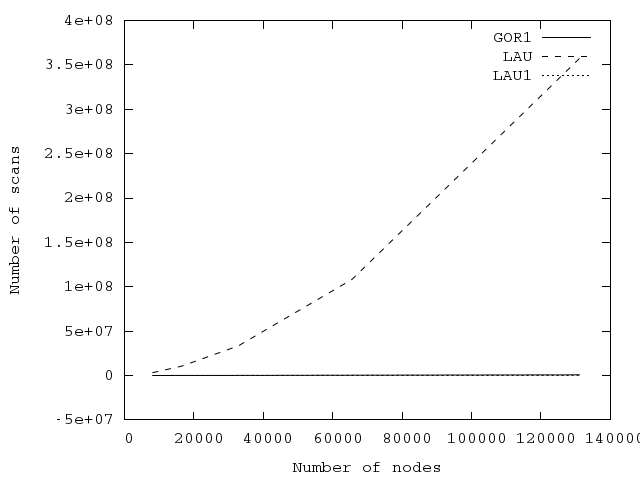
\includegraphics[width=\linewidth]{img/plot_acyc_neg.png}
\nolinebreak[4]
\\\footnotesize{Behavior of LAU, LAU1 and GOR1 on Acyc-Neg family.}
\end{center}

\begin{center}
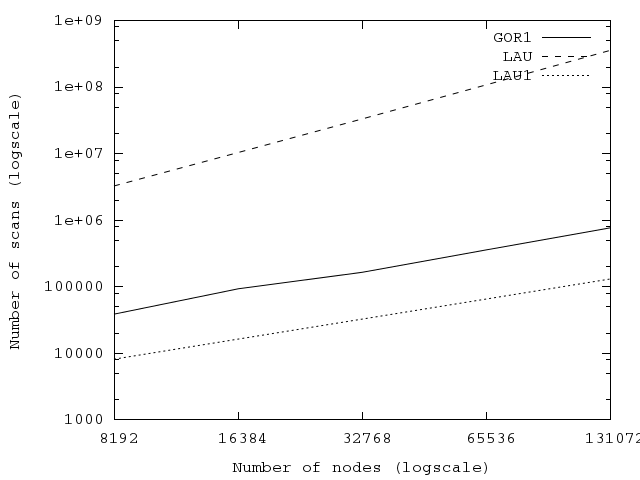
\includegraphics[width=\linewidth]{img/plot_acyc_neg_logscale.png}
\nolinebreak[4]
\\\footnotesize{Behavior of LAU, LAU1 and GOR1 on Acyc-Neg family (logarithmic scale on both axes).}
\end{center}

On Grid-NHard and Grid-PHard families (graphs with cycles designed to be hard for algorithms that exploit graph structure)
both LAU and LAU1 are very slow (though approximation suggests polynomial, not exponential fit),
while GOR1 is fast:

\begin{center}
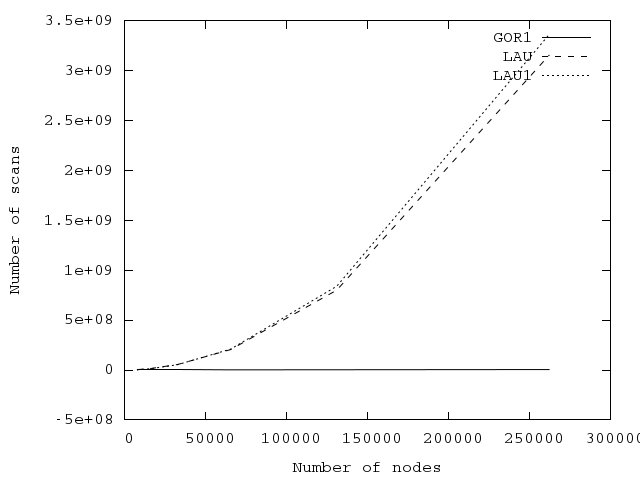
\includegraphics[width=\linewidth]{img/plot_grid_nhard.png}
\nolinebreak[4]
\\\footnotesize{Behavior of LAU, LAU1 and GOR1 on Grid-NHard family.}
\end{center}

\begin{center}
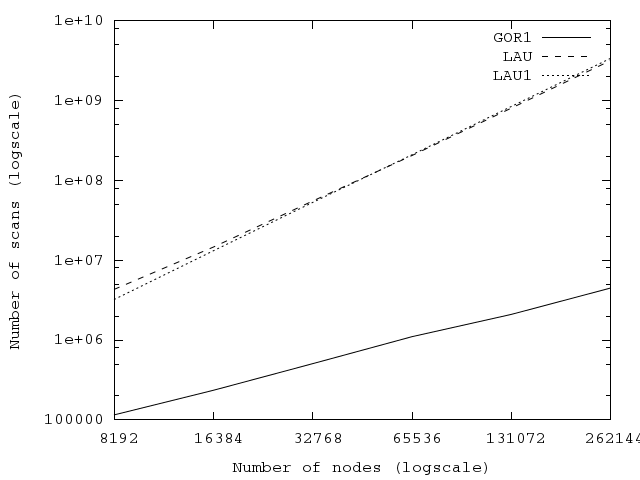
\includegraphics[width=\linewidth]{img/plot_grid_nhard_logscale.png}
\nolinebreak[4]
\\\footnotesize{Behavior of LAU, LAU1 and GOR1 on Grid-NHard family (logarithmic scale on both axes).}
\end{center}

On other graph families all three algorithms behave quite well;
it is strange that LAU is fast on Acyc-Pos family, while being so slow on Acyc-Neg family.
See also [NonPalXue00]: they study two modifications of GOR1, one of which is very close to LAU1,
and conjecture (without a proof) that worst-case complexity is exponential.

%\end{multicols}
%\begin{minipage}{\linewidth}
%\begin{center}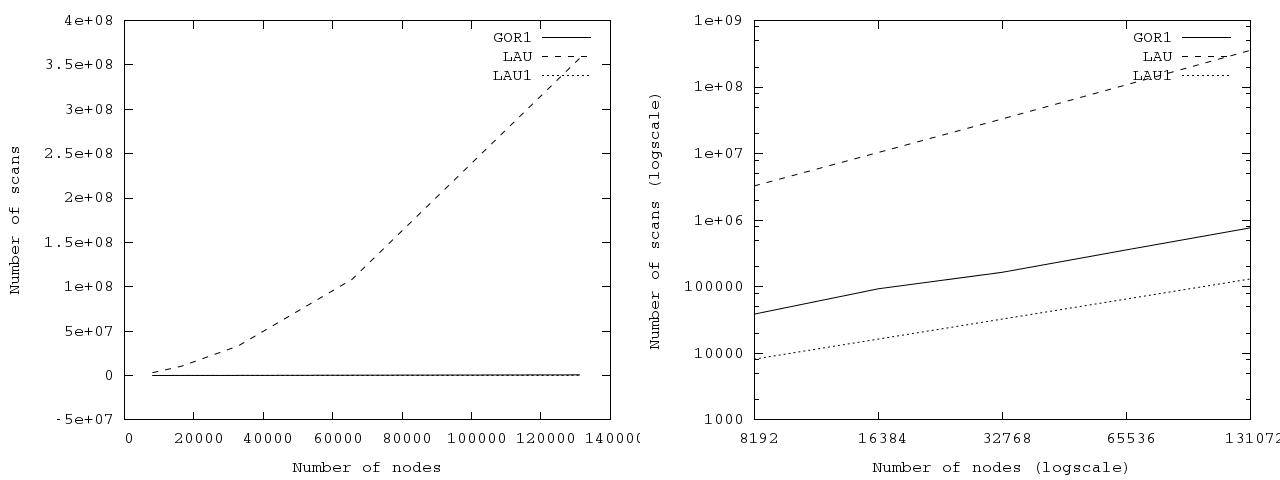
\includegraphics[width=\linewidth]{img/plot_acyc_neg_both.png}
%\\
%\footnotesize{Behavior of LAU, LAU1 and GOR algorithms on Acyc-Neg family
%(left -- normal scale, right -- logarithmic scale on both axes).}
%\end{center}
%\end{minipage}
%\begin{minipage}{\linewidth}
%\begin{center}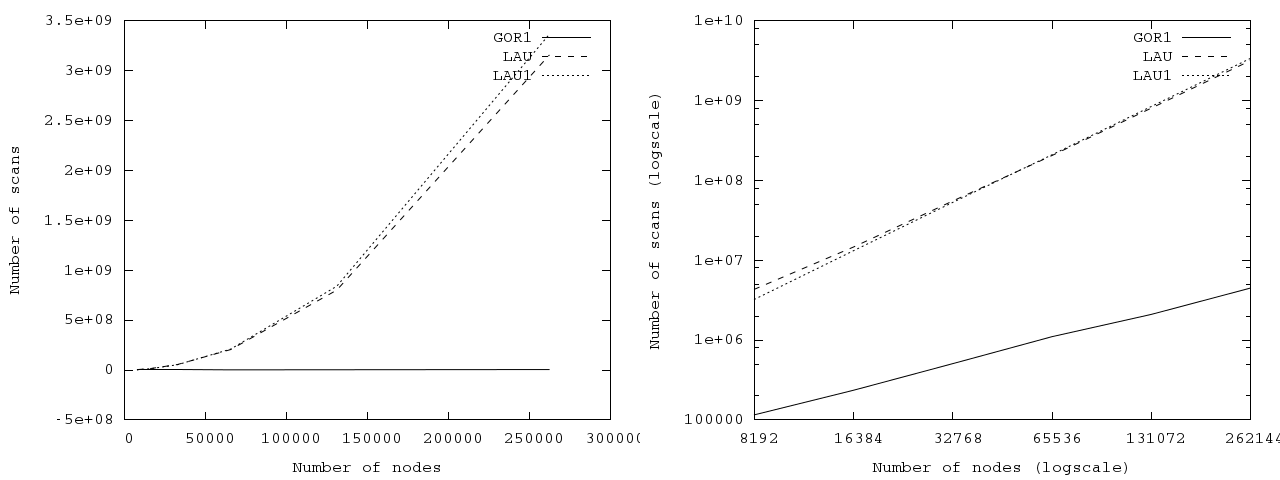
\includegraphics[width=\linewidth]{img/plot_grid_nhard_both.png}
%\\
%\footnotesize{Behavior of LAU, LAU1 and GOR algorithms on Grid-NHard family
%(left -- normal scale, right -- logarithmic scale on both axes).}
%\end{center}
%\end{minipage}
%\\
%\begin{multicols}{2}

\section{Disambiguation}\label{section_disambiguation}

In section \ref{section_tagged_extension} we defined disambiguation policy as strict partial order on the T-languge of the given TRE.
In practice T-language may be very large or infinite
and explicit listing of all ambiguous pairs is not an option; we need a comparison algorithm.
There are two main approaches: structure-based and value-based.
Structure-based disambiguation is guided by the order of operators in RE; tags play no role in it.
Value-based disambiguation is the opposite: it is defined in terms of maximization/minimization of certain tag parameters.
As a consequence, it has to deal with conflicts between different tags ---
a complication that never arises for structure-based approach.
Moreover, in value-based disambiguation different tags may have different rules and relations.
Below is a summary of two real-world policies supported by RE2C:
\\

\begin{itemize}
    \setlength{\parskip}{0.5em}
    \item Leftmost greedy.
        Match the longest possible prefix of the input string
        and take the \emph{leftmost path} through RE that corresponds to this prefix:
        in unions prefer left alternative, in iterations prefer re-iterating.

    \item POSIX.
        Each subexpression including the RE itself should match as early as possible
        and span as long as possible, while not violating the whole match.
        Subexpressions that start earlier in RE have priority over those starting later.
        Empty match is considered longer than no match;
        repeated empty match is allowed only for non-optional repetitions.
    \\
\end{itemize}

As we have already seen, a sufficient condition for efficient TNFA simulation is that the policy is prefix-based.
What about determinization?
In order to construct TDFA we must be able to fold loops:
if there is a nonempty loop in TNFA, determinization must eventually construct a loop in TDFA
(otherwise it won't terminate).
To do this, determinization must establish \emph{equivalnce} of two TDFA states.
%We cannot define equivalence as exact coincidence: if there is a loop, histories in one state are prefixes of histories in the other.
%But we can use a weaker definition:
From disambiguation point of view equivalence means that all ambiguities stemming from one state
are resolved in the same way as ambiguities stemming from the other.
However, we cannot demand exact coincidence of all state attributes engaged in disambiguation:
if there is loop, attributes in one state are extensions of those in the other state (and hence not equal).
Therefore we need to abstract away from absolute paths and define ``ambiguity shape'' of each state: relative order on all its configurations.
Disambiguation algorithm must be defined in terms of relative paths, not absolute paths.
Then we could compare states by their orders.
If disambiguation policy can be defined in this way, we call it \emph{foldable}.
\\

In subsequent sections we will formally define both policies in terms of comparison of ambiguous T-strings
and show that each policy is prefix-based and foldable.

\subsection{Leftmost greedy}

Leftmost greedy policy was extensively studied by many authors; we will refer to [Gra15], as their setting is very close to ours.
We can define it as lexicographic order on the set of all bitcodes corresponding to ambiguous paths
(see [Gra15], definition 3.25).
Let $\pi_1$, $\pi_2$ be two ambiguous paths which induce T-strings $x \Xeq \XT(\pi_1)$, $y \Xeq \XT(\pi_2)$
and bitcodes $a \Xeq \XB(\pi_1)$, $b \Xeq \XB(\pi_2)$.
Then $x \prec y$ iff $\prec_{lexicographic} (a, b)$:
\\

    $\prec_{lexicographic} (a_1 \dots a_n, b_1 \dots b_m)$
    \hrule
    \begin{enumerate}[leftmargin=0in]
        \smallskip
        \item[] for $i \Xeq \overline{1, min(n, m)}$:
        \begin{enumerate}
            \item[] if $a_i \!\neq\! b_i$ return $a_i \!<\! b_i$
        \end{enumerate}
        \item[] return $n \!<\! m$.
        \\
    \end{enumerate}
    \bigskip

This definition has one caveat: the existence of minimal element is not guaranteed for TRE that contain $\epsilon$-loops.
For example, TNFA for $\epsilon^+$ has infinitely many ambiguous paths with bitcodes
of the form $\widehat{0}^n \widehat{1}$, where $n \!\geq\! 0$,
and each bitcode is lexicographically less than the previous one.
Paths that contain $\epsilon$-loops are called \emph{problematic} (see [Gra15], definition 3.28).
If we limit ourselves to non-problematic paths (e.g. by cancelling loops in $\epsilon$-closure),
then the minimal element exists and bitcodes are well-ordered.
%The following lemma states an important property of bitcodes induced by paths gathered by $\epsilon$-closure:

\begin{XLem}\label{lemma_bitcodes}
Let $\Pi$ be a set of TNFA paths that have common start state, induce the same S-string and end in a core state.
Then the set of bitcodes induced by paths in $\Pi$ is prefix-free
(compare with [Gra15], lemma 3.1).

\medskip

Proof.
Consider paths $\pi_1$ and $\pi_2$ in $\Pi$,
and suppose that $\XB(\pi_1)$ is a prefix of $\XB(\pi_2)$.
Then $\pi_1$ must be a prefix of $\pi_2$: otherwise there is a state where $\pi_1$ and $\pi_2$ diverge,
and by TNFA construction all outgoing transitions from this state have different priorities,
which contradicts the equality of bitcodes.
Let $\pi_2 \Xeq \pi_1 \pi_3$.
Since $\XS(\pi_1) \Xeq \XS(\pi_2)$, and since $\XS(\rho\sigma) \Xeq \XS(\rho)\XS(\sigma)$ for arbitrary path $\rho\sigma$,
it must be that $\XS(\pi_3) \Xeq \epsilon$.
The end state of $\pi_2$ is a core state: by TNFA construction it has no outgoing $\epsilon$-transitions.
But it is also the start state of $\epsilon$-path $\pi_3$, therefore $\pi_3$ is an empty path and $\pi_1 \Xeq \pi_2$.
$\square$
\end{XLem}

From Lemma \ref{lemma_bitcodes} it easily follows that leftmost greedy disambiguation is prefix-based.
Consider ambiguous paths $\pi_1$, $\pi_2$ and arbitrary suffix $\pi_3$,
and let $\XB(\pi_1) \Xeq a$, $\XB(\pi_2) \Xeq b$, $\XB(\pi_3) \Xeq c$.
Note that $\XB(\rho\sigma) \Xeq \XB(\rho)\XB(\sigma)$ for arbitrary path $\rho\sigma$,
therefore $\XB(\pi_1\pi_3) \Xeq ac$ and $\XB(\pi_2\pi_3) \Xeq bc$.
If $a \Xeq b$, then $ac \Xeq bc$.
Otherwise, without loss of generality let $a \prec_{lexicographic} b$: since $a$, $b$ are prefix-free, $ac \prec_{lexicographic} bc$
(compare with [Gra15], lemma 2.2).
\\

From Lemma \ref{lemma_bitcodes} it also follows that leftmost greedy disambiguation is foldable:
prefix-free bitcodes can be compared incrementally on each step of simulation.
We define ``ambiguity shape'' of TDFA state as lexicographic order on bitcodes of all paths represented by configurations
(compare with [Gra15], definition 7.14).
The number of different weak orderings of $n$ elements is finite, therefore determinization terminates
(this number equals $\sum_{k=0}^n \Xstirling{n}{k} k!$, also known as the \emph{ordered Bell number} [??]).
Order on configurations is represented with ordinal numbers assigned to each configuration.
Ordinals are initialized to zero and then updated on each step of simulation by comparing bitcodes.
Bitcodes are compared incrementally:
first, by ordinals calculated on the previous step, then by bitcode fragments added by the $\epsilon$-closure.
\\

%\begin{minipage}{\linewidth}
    $\prec_{leftmost \Xund greedy} ((n, a), (m, b))$
    \hrule
    \begin{enumerate}[leftmargin=0in]
        \smallskip
        \item[] if $n \!\neq\! m$ return $n \!<\! m$
        \item[] return $\prec_{lexicographic} (a, b)$
        \\
    \end{enumerate}
%\end{minipage}

    \bigskip

%\begin{minipage}{\linewidth}
    $ordinals (\{(q_i, o_i, x_i)\}_{i=1}^n)$
    \hrule
    \begin{enumerate}[leftmargin=0in]
    \smallskip
        \item[] $\{(p_i, B_i)\} \Xset $ sort $\{(i, (o_i, x_i))\}$ by second component \\
            \hphantom{hspace{2em}} using $\prec_{leftmost \Xund greedy}$ as comparator
        \item[] $\widetilde{o}_{p_1 t} \Xset 0, \; j \Xset 0$
        \item[] for $i \Xeq \overline{2, n}$:
        \begin{enumerate}
            \item[] if $B_{i-1} \!\neq\! B_i: j \Xset j \!+\! 1$
            \item[] $\widetilde{o}_{p_i t} \Xset j$
        \end{enumerate}
        \item[] return $\{(q_i, \widetilde{o}_i, x_i)\}_{i=1}^n$
        \\
    \end{enumerate}
%\end{minipage}

    \bigskip

In practice explicit calculation of ordinals and comparison of bitcodes is not necessary:
if we treat TDFA states as ordered sets,
sort TNFA transitions by their priority
and define $\epsilon$-closure as a simple depth-first search,
then the first path that arrives at any state would be the leftmost.
This approach is taken in e.g. [Karper].
Since tags are not engaged in disambiguation,
we can use paired tags that represent capturing parenthesis, or just standalone tags --- this makes no difference with leftmost greedy policy.

\subsection{POSIX}

POSIX policy is defined in [??]; [Fow] gives a comprehensible interpretation of it.
We will give a formal interpretation in terms of tags;
it was first described by Laurikari in [Lau01], but the key idea must be absolutely attributed to Kuklewicz [??].
He never fully formalized his algorithm, and our version slightly deviates from the informal description,
so all errors should be attributed to the author of this paper.
Fuzz-testing RE2C against Regex-TDFA revealed no difference in submatch extraction
(see section ?? for details).
\\

Consider an arbitrary RE without tags,
and suppose that parenthesized subexpressions are marked for submatch extraction.
We start by enumerating all subexpressions according to POSIX standard:

    \begin{Xdef}
    For a given RE $e$, its \emph{indexed RE (IRE)} is $(\widetilde{e}, n \!-\! 1)$,
    where $(\widetilde{e}, n) \Xeq \XI(e, 1)$
    and $\XI$ is defined as follows:
    \begin{align*}
        \XI(\emptyset, i) &= ((i, \emptyset), i \!+\! 1) \\
        \XI(\epsilon, i) &= ((i, \epsilon), i \!+\! 1) \\
        \XI(\alpha, i) &= ((i, \alpha), i \!+\! 1) \\
        \XI(e_1 | e_2, i) &= ((i, \widetilde{e_1} | \widetilde{e_2}), k) \\
            \text{where }
            & (\widetilde{e_1}, j) \Xeq \XI(e_1, i \!+\! 1),
            \; (\widetilde{e_2}, k) \Xeq \XI(e_2, j \!+\! 1) \\
        \XI(e_1 e_2, i) &= ((i, \widetilde{e_1} \widetilde{e_2}), k) \\
            \text{where }
            & (\widetilde{e_1}, j) \Xeq \XI(e_1, i \!+\! 1),
            \; (\widetilde{e_2}, k) \Xeq \XI(e_2, j \!+\! 1) \\
        \XI(e^{n,m}, i) &= ((i, \widetilde{e}^{n,m}), j) \\
            \text{where } & (\widetilde{e}, j) \Xeq \XI(e, i \!+\! 1)
    \end{align*}
    $\square$
    \end{Xdef}

Next, we rewrite IRE into TRE by rewriting each indexed subexpression $(i, e)$
into tagged subexpression $t_1 e \, t_2$, where $t_1 \Xeq 2i \!-\! 1$ is the \emph{start tag}
and $t_2 \Xeq 2i$ is the \emph{end tag}.
Tags that correspond to iteration subexpressions are called \emph{orbit} tags.
\\

Strictly speaking, IRE is not necessary: it's just a consise way of enumerating tags.
For example, RE $a^* (b | \epsilon)$ corresponds to IRE
$(1,
    (2, (3, a)^*)
    (4, (5, b) | (6, \epsilon))
)$
and to TRE
$(1\,
    3\, (5\, a \,6)^* \,4\,
    7\, (9\, b \,10 | 11\, \epsilon \,12) 8\,
2)$.
\\

POSIX disambiguation is hierarchical:
it starts with the first subexpression and traverses subexpressions in order of their indices.
For each subexpression it compares positions of start and end tags in the two given T-strings.
Positions are called \emph{offsets}; each offset is either $\varnothing$ (if the occurence of tag is negative),
or equal to the number of $\Sigma$-symbols before this occurence.
The sequence of offsets is called \emph{history}.
Each history consists of one or more \emph{subhistories}:
they correspond to longest continuous substrings not interrupted by tags of subexpressions with lower indices.
For non-iteration subexpressions subhistories contain exactly one offset;
for iteration subexpressions they are either $\varnothing$, or may contain multiple non-$\varnothing$ offsets.
If disambiguation is between T-string prefixes, then the last subhistory may be incomplete or empty.
The following algorithm constructs a list of subhistories for the given T-string (possibly prefix) and tag.
Its complexity is $O(n)$, since it processes each symbol at most once:
\\

%\begin{minipage}{\linewidth}
    $history(a_1 \dots a_n, t)$
    \hrule
    \begin{enumerate}[leftmargin=0in]
        \smallskip
        \item[] $U \Xset \{ u \mid u < 2 \lceil t / 2 \rceil \!-\! 1 \}$
        \item[] $i \Xset 1, \; j \Xset 1, \; p \Xset 0$

        \item[] while $true$
        \begin{enumerate}

            \item[] while $i \leq n$ and $a_i \!\not\in\! \{t, \Xbar{t}\}$
            \begin{enumerate}
                \item[] if $a_i \Xin \Sigma: p \Xset p \!+\! 1$
                \item[] $i \Xset i \!+\! 1$
            \end{enumerate}

            \item[] while $i \leq n$ and $a_i \!\not\in\! (U \cup \Xbar{U})$
            \begin{enumerate}
                \item[] if $a_i \Xin \Sigma: p \Xset p \!+\! 1$
                \item[] if $a_i \Xeq t: A_j \Xset A_j p$
                \item[] if $a_i \Xeq \Xbar{t}: A_j \Xset A_j \varnothing$
                \item[] $i \Xset i \!+\! 1$
            \end{enumerate}

            \item[] if $i \!>\! n$ break
            \item[] $j \Xset j \!+\! 1$

        \end{enumerate}
        \item[] return $A_1 \dots A_j$
    \end{enumerate}
%\end{minipage}

    \bigskip

Because of the hierarchical structure of POSIX disambiguation, if comparison reaches $i$-th subexpression,
it means that all subexpressions with lower indices have already been considered and their histories coincide.
Consequently for start and end tags of $i$-th subexpression
the number of subhistories in the compared T-strings must be equal.
If comparison is between prefixes, last subhistory of start tag may contain one more offset than last suhistory of end tag:
in this case we assume that the missing offset if $\infty$ (as it must be greater than any offset in this history).
Given all that, POSIX disambiguation for TRE with $N$ subexpressions is defined as follows:
\\

%\begin{minipage}{\linewidth}
    $\prec_{POSIX}(x, y)$
    \hrule
    \begin{enumerate}[leftmargin=0in]
        \smallskip
        \item[] for $t \Xeq \overline{1, N}$:
        \begin{enumerate}
            \item[] $A_1 \dots A_n \Xset history(x, 2t \!-\! 1)$
            \item[] $C_1 \dots C_n \Xset history(x, 2t)$
            \item[] $B_1 \dots B_n \Xset history(y, 2t \!-\! 1)$
            \item[] $D_1 \dots D_n \Xset history(y, 2t)$
            \item[] for $i \Xeq \overline{1, n}$:
            \begin{enumerate}
                \item[] let $A_i \Xeq a_1 \dots a_m$, $C_i \Xeq c_1 \dots c_{\widetilde{m}}$
                \item[] let $B_i \Xeq b_1 \dots b_k$, $D_i \Xeq d_1 \dots d_{\widetilde{k}}$
                \item[] if $\widetilde{m} \!<\! m: c_m \Xset \infty$
                \item[] if $\widetilde{k} \!<\! k: d_k \Xset \infty$
                \item[] for $j \Xeq \overline{1, min(m, k)}$:
                \begin{enumerate}
                    \item[] if $a_j \!\neq\! b_j$ return $a_j \!<\! b_j$
                    \item[] if $c_j \!\neq\! d_j$ return $c_j \!>\! d_j$
                \end{enumerate}
                \item[] if $m \!\neq\! k$ return $m \!<\! k$
            \end{enumerate}
        \end{enumerate}
        \item[] return $false$
        \\
    \end{enumerate}
%\end{minipage}

    \bigskip

It's not hard to show that $\prec_{POSIX}$ is prefix-based.
Consider $t$-th iteration of the algorithm and let $s \Xeq 2t \!-\! 1$ be the start tag,
$history(x, s) \Xeq A_1 \dots A_n$ and $history(y, s) \Xeq B_1 \dots B_n$.
The value of each offset depends only on the number of preceding $\Sigma$-symbols,
therefore for an arbitrary suffix $z$ we have:
$history(xz, s) \Xeq A_1 \dots A_{n-1} A'_n C_1 \dots C_n$ and
$history(yz, s) \Xeq B_1 \dots B_{n-1} B'_n C_1 \dots C_n$,
where $A'_n \Xeq A_n c_1 \dots c_m$, $B'_n \Xeq B_n c_1 \dots c_m$.
The only case when $z$ may affect comparison is when $m \!\geq\! 1$ and one history is a proper prefix of the other:
$A_i \Xeq B_i$ for all $i \Xeq \overline{1,n-1}$ and (witout loss of generality) $B_n \Xeq A_n b_1 \dots b_k$.
Otherwise either histories are equal, or comparison terminates before reaching $c_1$.
Let $d_1 \dots d_{k+m} \Xeq b_1 \dots b_k c_1 \dots c_m$.
None of $d_j$ can be $\varnothing$, because $n$-th subhistory contains multiple offsets.
Therefore $d_j$ are non-decreasing and $d_j \!\leq\! c_j$ for all $j \Xeq \overline{1, m}$.
Then either $d_j \!<\! c_j$ at some index $j \!\leq\! m$, or $A'_n$ is shorter than $B'_n$; in both cases comparison result is unchanged.
The same reasoning holds for the end tag.
\\

It is less evident that $\prec_{POSIX}$ is foldable:
the rest of this chapter is a long and tiresome justification of Kuklewicz algorithm
(with a coulple of modifications and ideas by the author).
\\

First, we simplify $\prec_{POSIX}$.
It makes a lot of redundant checks:
for adjacent tags the position of the second tag is fixed on the position of the first tag.
In particular, comparison of the start tags $a_j$ and $b_j$ is almost always redundant.
If $j \!>\! 1$, then $a_j$ and $b_j$ are fixed on $c_{j-1}$ and $d_{j-1}$, which have been compared on the previous iteration.
If $j \Xeq 1$, then $a_j$ and $b_j$ are fixed on some higher-priority tag which has already been checked, unless $t \Xeq 1$.
The only case when this comparison makes any difference is when $j \Xeq 1$ and $t \Xeq 1$:
the very first position of the whole match.
In order to simplify further discussion we will assume that the match is anchored;
otherwise one can handle it as a special case of comparison algorithm.
The simplified algorithm looks like this:
\\

%\begin{minipage}{\linewidth}
    $\prec_{POSIX}(x, y)$
    \hrule
    \begin{enumerate}[leftmargin=0in]
        \smallskip
        \item[] for $t \Xeq \overline{1, N}$:
        \begin{enumerate}
            \item[] $A_1 \dots A_n \Xset history(x, 2t)$
            \item[] $B_1 \dots B_n \Xset history(y, 2t)$
            \item[] for $i \Xeq \overline{1, n}$:
            \begin{enumerate}
                \item[] if $A_i \!\neq\! B_i: return \prec_{subhistory} (A_i, B_i)$
            \end{enumerate}
        \end{enumerate}
        \item[] return $false$
        \\
    \end{enumerate}
%\end{minipage}

    \bigskip

%\begin{minipage}{\linewidth}
    $\prec_{subhistory} (a_1 \dots a_n, b_1 \dots b_m)$
    \hrule
    \begin{enumerate}[leftmargin=0in]
        \smallskip
        \item[] for $i \Xeq \overline{1, min(n, m)}$:
        \begin{enumerate}
            \item[] if $a_i \!\neq\! b_i$ return $a_i \!>\! b_i$
        \end{enumerate}
        \item[] return $n \!<\! m$.
        \\
    \end{enumerate}
%\end{minipage}

    \bigskip

Next, we explore the structure of ambigous paths that contain multiple subhistories
and show that (under ceratin conditions) such paths can be split into ambiguous subpaths,
one per each subhistory.
\\

\begin{XLem}\label{lemma_path_decomposition}
For a POSIX TRE $e$,
if $a$, $b$ are ambiguous paths in TNFA $\XN(e)$, such that $\XT(a) \Xeq x$, $\XT(b) \Xeq y$,
$t$ is a tag such that $history(x, u) \Xeq history(y, u)$ for all $u \!<\! t$
and $history(x, t) \Xeq A_1 \dots A_n$, $history(y, t) \Xeq B_1 \dots B_n$,
then $a$, $b$ can be decomposed into path segments $a_1 \dots a_n$, $b_1 \dots b_n$,
such that for all $i \!\leq\! n$ paths $a_1 \dots a_i$, $b_1 \dots b_i$ are ambiguous
and $history(\XT(a_1 \dots a_i), t) \Xeq A_1 \dots A_i$, $history(\XT(b_1 \dots b_i), t) \Xeq B_1 \dots B_i$.
\\
\\
Proof is by induction on $t$ and relies on the construction of TNFA given in Theorem \ref{theorem_tnfa}.
Induction basis is $t \Xeq 1$ and $t \Xeq 2$ (start and end tags of the topmost subexpression): let $n \Xeq 1$, $a_1 \Xeq a$, $b_1 \Xeq b$.
Induction step: suppose that lemma is true for all $u \!<\! t$,
and for $t$ the conditions of lemma are satisfied.
Let $r$ be the start tag of a subexpression in which $t$ is immediately enclosed.
Since $r \!<\! t$, the lemma is true for $r$ by inductive hypothesis;
%let $history(x, r) \Xeq C_1 \dots C_m$, $history(y, r) \Xeq D_1 \dots D_m$ and
let $c_1 \dots c_m$, $d_1 \dots d_m$ be the corresponding path decompositions.
Each subhistory of $t$ is covered by some subhistory of $r$ (by definition $history$ doesn't break at lower-priority tags),
therefore decompositions $a_1 \dots a_n$, $b_1 \dots b_n$ can be constructed as a refinement of $c_1 \dots c_m$, $d_1 \dots d_m$.
If $r$ is a non-orbit tag, each subhistory of $r$ contains exactly one subhistory of $t$
and the refinement is trivial: $n \Xeq m$, $a_i \Xeq c_i$, $b_i \Xeq d_i$.
Otherwise, $r$ is an orbit tag and single subhistory of $r$ may contain multiple subhistories of $t$.
Consider path segments $c_i$ and $d_i$:
since they have common start and end states, and since they cannot contain tagged transitions with higher-priority tags,
both must be contained in the same subautomaton of the form $F^{k,l}$ (possibly $l \Xeq \infty$).
This subautomaton itself consists of one or more subautomata for $F$ each starting with an $r$-tagged transition;
let the start state of each subautomaton be a breaking point in the refinement of $c_i$ and $d_i$.
By construction of TNFA the number of iterations through $F^{k,l}$ uniquely determins the order of subautomata traversal
(automaton corresponding to $(j \!+\! 1)$-th iteration is only reachable from the one corresponding to $j$-th iteration).
Since $history(x, r) \Xeq history(y, r)$, the number of iterations is equal and
therefore breaking points coincide.
$\square$
\end{XLem}

Lemma \ref{lemma_path_decomposition} has the following implication.
Suppose that at $p$-th step of TNFA simulation we are comparing histories $A_1 \dots A_n$, $B_1 \dots B_n$.
Let $j \!\leq\! n$ be the greatest index such that $A_1 \dots A_j$, $B_1 \dots B_j$ end before $p$-th position in the input string
(it is the same index for both histories because higher-priority tags coincide).
Then $A_i \Xeq B_i$ for all $i \!\leq\! j$:
by Lemma \ref{lemma_path_decomposition} $A_1 \dots A_j$, $B_1 \dots B_j$
correspond to ambiguous subpaths which must have been compared on some previous step of the algorithm.
This means that we only need to compare $A_{j+1} \dots A_n$ and $B_{j+1} \dots B_n$.
Of them only $A_{j+1}$ and $B_{j+1}$ may start before $p$-th position in the input string:
all other subhistories belong to current $\epsilon$-closure (though $A_n$, $B_n$ may not end in it).
Therefore between steps of simulation we need to remeber only the last (possibly incomplete) subhistory of each tag.
\\

Now we can define ``ambiguity shape'' of TDFA state:
we define it as a set of orders, one for each tag, on the last subhistories of this tag in this state.
Of course, comparison only makes sense for subhistories that correspond to ambiguous paths and prefixes of ambiguous paths,
and in general we do not know which prefixes will cause ambiguity on subsequent steps.
Therefore some comparisons may be meaningless, incorrect and unjustified.
However, they do not affect valid comparisons,
and they do not cause disambiguation errors: their results are never used.
At worst they can prevent state merging.
As with leftmost greedy policy, the number of different orders is finite
and therefore determinization terminates.
\\

Consider subhistories for which comparison is valid.
Comparison algorithm differs for orbit and non-orbit tags.
Orbit subhistories can be compared incrementally:
if at some step we determine that $A \prec B$, then it will be true ever after, no matter what values are added to $A$ and $B$.
(This can be proven by induction on the number of steps
and using the fact that $\varnothing$ can be added only at the first step,
by TNFA construction for the case of zero iterations).
Therefore we can use the results of comparison on the previous step and compare only the added parts of subhistories.
For non-orbit tags incremental comparison doesn't work:
subhistories consist of a single value, but different paths may discover it at different steps,
and the later value may turn to be either $\varnothing$ or not.
However, a single value cannot be spread across multiple steps:
it either belongs to current $\epsilon$-closure or to some earlier step.
If both values belong to earlier steps, we can use results of the previous comparison;
it they both belong to $\epsilon$-closure, they are equal;
otherwise the one from the $\epsilon$-closure is better.
\\

Orders on configurations are represented with vectors of ordinal numbers (one per tag) assigned to each configuration.
Ordinals are initialized to zero and updated on each step of simulation by comparing tag histories.
Histories are compared using ordinals calculated on the previous step and T-string fragments added by $\epsilon$-closure.
Ordinals are assigned in decreasing order, so that they can be compared in the same way as offsets: greater means better.
\\

%\begin{minipage}{\linewidth}
    $ordinals (\{(q_i, o_i, x_i)\}_{i=1}^n)$
    \hrule
    \begin{enumerate}[leftmargin=0in]
        \smallskip
        \item[] for $t \Xeq \overline{1, N}$:
        \begin{enumerate}
            \item[] for $i \Xeq \overline{1, n}$:
            \begin{enumerate}
                \item[] $A_1 \dots A_m \Xset \epsilon \Xund history(x_i, t)$
                \item[] $B_i \Xset A_m$
                \item[] if $m \Xeq 1$ and ($t$ is an orbit tag or $B_i \Xeq \epsilon$)
                \begin{enumerate}
                    \item[] $B_i \Xset o_{i t} B_i$
                \end{enumerate}
            \end{enumerate}
            \smallskip
            \item[] $\{(p_i, C_i)\} \Xset $ sort $\{(i, B_i)\}$ by second component \\
                \hphantom{\quad} using inverted $\prec_{subhistory}$ as comparator
            \item[] $\widetilde{o}_{p_1 t} \Xset 0, \; j \Xset 0$
            \item[] for $i \Xeq \overline{2, n}$:
            \begin{enumerate}
                \item[] if $C_{i-1} \!\neq\! C_i: j \Xset j \!+\! 1$
                \item[] $\widetilde{o}_{p_i t} \Xset j$
            \end{enumerate}
        \end{enumerate}
        \smallskip
        \item[] return $\{(q_i, \widetilde{o}_i, x_i)\}_{i=1}^n$
        \\
    \end{enumerate}
%\end{minipage}

    \bigskip

The $history$ algorithm is modified so that it works on T-string fragments added by the $\epsilon$-closure.
Non-$\varnothing$ offsets are set to $\infty$, since all tags in the $\epsilon$-closure have the same position
which must be greater than any ordinal calculated on the previous step.
\\

%\begin{minipage}{\linewidth}
    $\epsilon \Xund history (a_1 \dots a_n, t)$
    \hrule
    \begin{enumerate}[leftmargin=0in]
        \smallskip
        \item[] $U \Xset \{ u \mid u < 2 \lceil t / 2 \rceil \!-\! 1 \}$
        \item[] $i \Xset 1, \; j \Xset 1$

        \item[] while $true$
        \begin{enumerate}
            \item[] while $i \leq n$ and $a_i \!\not\in\! (U \cup \Xbar{U})$
            \begin{enumerate}
                \item[] if $a_i \Xeq t: A_j \Xset A_j \infty$
                \item[] if $a_i \Xeq \Xbar{t}: A_j \Xset A_j \varnothing$
                \item[] $i \Xset i \!+\! 1$
            \end{enumerate}

            \item[] if $i \!>\! n$ break
            \item[] $j \Xset j \!+\! 1$

            \item[] while $i \leq n$ and $a_i \!\not\in\! \{t, \Xbar{t}\}$
            \begin{enumerate}
                \item[] $i \Xset i \!+\! 1$
            \end{enumerate}

        \end{enumerate}
        \item[] return $A_1 \dots A_j$
    \end{enumerate}
%\end{minipage}

    \bigskip

Finally, disambiguation algorithm is redefined in terms of ordinals and added T-string fragments:
\\

%\begin{minipage}{\linewidth}
    $\prec_{POSIX}((ox, x), (oy, y))$
    \hrule
    \begin{enumerate}[leftmargin=0in]
        \smallskip
        \item[] for $t \Xeq \overline{1, N}$:
        \begin{enumerate}
            \item[] $A_1 \dots A_n \Xset \epsilon \Xund history(x, 2t), \; a \Xset ox_{2t}$
            \item[] $B_1 \dots B_n \Xset \epsilon \Xund history(y, 2t), \; b \Xset oy_{2t}$

            \item[] if $2t$ is an orbit tag:
            \begin{enumerate}
                \item[] $A_1 \Xset a A_1$
                \item[] $B_1 \Xset b B_1$
            \end{enumerate}
            \item[] else
            \begin{enumerate}
                \item[] if $A_1 \Xeq \epsilon: A_1 \Xset a$
                \item[] if $B_1 \Xeq \epsilon: B_1 \Xset b$
            \end{enumerate}

            \item[] for $i \Xeq \overline{1, n}$:
            \begin{enumerate}
                \item[] if $A_i \!\neq\! B_i: return \prec_{subhistory} (A_i, B_i)$
            \end{enumerate}

        \end{enumerate}
        \item[] return $false$
        \\
    \end{enumerate}
%\end{minipage}

    \bigskip

So far we have treated all subexpressions uniformly as if they were marked for submatch extraction.
In practice most of them are not: we can reduce the amount of tags by dropping all tags in subexpressions without nested submatches
(since no other tags depend on them).
However, all the hierarchy of tags from the topmost subexpression down to each submatch must be preserved,
including \emph{fictive} tags that don't correspond to any submatch and exist purely for disambiguation purposes.
They are probably not many: POSIX RE use the same operator for grouping and submatching,
and compound expressions usually need grouping to override operator precedence,
so it is uncommon to construct a large RE without submatches.
%(otherwise union cannot be enclosed in concatenation and repetition of non-atomic subexpressions cannot be used at all).
However, fictive tags must be inserted into RE; neither Laurikari nor Kuklewicz mention it,
but both their libraries seem to do it (judging by the source code).
\\

In this respect TDFA-based matchers have an advantage over TNFA-based ones:
disambiguation happens at determinization time,
and afterwards we can erase all fictive tags -- the resulting TDFA will have no overhead.
However, if it is necessary to reduce the amount of tags at all costs (even at disambiguation time),
then fictive tags can be dropped and the algorithm modified as follows.
Each submatch should have two tags (start and end)
and repeated submatches should also have a third (orbit) tag.
Start and end tags should be maximized, if both conflicting subhistories are non-$\varnothing$;
otherwise, if only one is $\varnothing$, leftmost path should be taken;
if both are $\varnothing$, disambiguation should continue with the next tag.
Orbit tags obey the same rules as before.
The added complexity is caused by the possible absence of tags in the left part of union and concatenation.
We won't go into further details, as the modified algorithm is probably not very useful;
but an exprimental implementation in RE2C passed all the tests in [??].
Correctness proof might be based on the limitations of POSIX RE due to the coupling of groups and submatches.

\section{Determinization}\label{section_determinization}

When discussing TNFA simulation we paid little attention to tag value functions:
decomposition must wait until disambiguation, which is defined on T-strings,
and in general this means waiting until the very end of simulation.
However, since then we have studied leftmost greedy and POSIX policies more closely
and established that both are prefix-based and foldable.
This makes them suitable for determinization, but also opens possibilities for more efficient simulation.
In particular, there's no need to remember the whole T-string for each active path:
we only need ordinals and the most recent fragment added by the $\epsilon$-closure.
All the rest can be immediately decomposed into tag value function (or any other suitable representation).
Consequently, we extend configurations with vectors of \emph{tag values}:
in general, each value is an offset list of arbitrary length,
but in practice values may be single offsets or anything else.
\\

Laurikari determinization algorithm has the same basic principle as the usual powerset construction:
simulation of nondeterministic automaton on all possible inputs combined with merging of equivalent states.
The most tricky part is merging: extended configuration sets are no longer equal, as they contain absolute tag values.
%(in fact, they cannot coincide in case of tagged non-empty loops in TNFA).
In section \ref{section_disambiguation} we solved similar problem with respect to disambiguation
by moving from absolute T-strings to relative ordinals.
However, this wouldn't work with tag values, as we need the exact offsets.
Laurikari resolved this predicament using \emph{references}:
he noticed that we can represent tag values as cells in ``memory'' and address each value by reference to the cell that holds it.
If states $X$ and $Y$ are equal up to renaming of references,
then we can convert $X$ to $Y$ by copying the contents of cells in $X$ to the cells in $Y$.
The number of different cells needed at each step is finite:
it is bounded by the number of tags times the number of configurations in the given state.
Therefore ``memory'' can be modelled as a finite set of \emph{registers},
which brings us to the following definition of TDFA:

    \begin{Xdef}
    \emph{Tagged Deterministic Finite Automaton (TDFA)}
    is a structure $(\Sigma, T, \YQ, \YF, Q_0, R, \delta, \zeta, \eta, \iota)$, where:
    \begin{itemize}
    \setlength{\parskip}{0.5em}
        \item[] $\Sigma$ is a finite set of \emph{symbols} (\emph{alphabet})
        \item[] $T$ is a finite set of \emph{tags}
        \item[] $\YQ$ is a finite set of \emph{states}
        \item[] $\YF \subseteq \YQ$ is the set of \emph{final} states
        \item[] $Q_0 \in \YQ$ is the \emph{initial} state
        \item[] $R$ is a finite set of \emph{registers}
        \item[] $\delta: \YQ \times \Sigma \to \YQ$ is the \emph{transition} function
        \item[] $\zeta: \YQ \times \Sigma \times R \to R \times \YB^*$ \\
            is the \emph{register update} function
        \item[] $\eta: \YF \times R \to R \times \YB^*$ \\
            is the \emph{register finalize} function
        \item[] $\iota: R \to R \times \YB^*$ \\
            is the \emph{register initialize} function
    \end{itemize}
    where $\YB$ is the boolean set $\{0,1\}$.
    $\square$
    \end{Xdef}

Operations on registers have the form $r_1 \Xeq r_2 \cdot x$, where $x$ is a (possibly empty) boolean string
and $1$, $0$ denote \emph{current position} and \emph{default value}.
For example, $r_1 \Xeq 0$ means ``set $r_1$ to default value'',
$r_1 \Xeq r_2$ means ``copy $r_2$ to $r_1$'' and
$r_1 \Xeq r_1 1 1$ means ``append current position to $r_1$ twice''.
\\

TDFA definition looks very similar to the definition of
\emph{deterministic streaming string transducer (DSST)}, described by Alur and Cerny in [AluCer11].
Indeed, the two kinds of automata are similar and have similar applications: DSSTs are used for RE parsing in [Gra15].
However, their semantics is different: TDFA operates on tag values, while DSST operates on strings of the output language.
What is more important, DSST is \emph{copyless}:
its registers can be only \emph{moved}, not \emph{copied}.
TDFA violates this restriction, but this doesn't affect its performance as long as registers hold scalar values.
Fortunately, it is always possible to represent tag values as scalars
(single offsets are obviously scalar, and offset lists form a \emph{prefix tree} that can be stored as an array of pointers to parent,
as suggested in [Karper]).
\\

TDFA can be constructed in two slightly different ways
depending on whether we associate $\epsilon$-closure of each state with the \emph{incoming} transition,
or with all \emph{outgoing} transitions.
For the usual powerset construction it makes no difference, but things change in the presence of tagged transitions.
In the former case register operations are associated with the \emph{incoming} transition and should be executed \emph{after} it.
In the latter case they belong to each \emph{outgoing} transition and should be executed \emph{before} it,
which means that we can exploit the \emph{lookahead} symbol to filter out only the relevant part of $\epsilon$-closure:
pick only those $\epsilon$-paths which end states have transitions on the lookahead symbol.
This leaves out many useless register operations:
intuituvely, we delay their application until the right lookahead symbol shows up.
However, state mapping becomes more complex:
since the operations are delayed,
their effect on each state is not reflected in configurations at the time of mapping.
In order to ensure state equivalence we must additionaly demand exact coincidence of delayed operations.
\\

The two ways of constructing TDFA resemble slightly of LR(0) and LR(1) automata; we call them TDFA(0) and TDFA(1).
Indeed, we can define \emph{conflict} as a situation when tag has at least two different values in the given state.
Tags that induce no conflicts are \emph{deterministic};
the maximal number of different values per state is the tag's \emph{degree of nondeterminism}.
Accordingly, \emph{tag-deterministic} RE are those for which it is possible to build TDFA without conflicts.
As with LR(0) and LR(1), many RE are tag-deterministic with respesct to TDFA(1), but not TDFA(0).
Unlike LR automata, TDFA with conflicts are correct, but they can be very inefficient:
%tags with high degree of nondeterminizm induce a lot of register operations.
the higher tag's degree of nondeterminism, the more registers it takes to hold its values,
and the more operations are required to manage these registers.
Determinstic tags need only a single register and can be implemented without copy operations.
\\

Laurikari used TDFA(0); we study both methods and argue that TDFA(1) is better.
Determinization algorithm is designed in a way that can handle both types of automata in a uniform way.
States are sets of configurations $(q, v, o, x)$,
where $q$ is a core TNFA state, $v$ is a vector of registers that hold tag values, $o$ is the ordinal
and $x$ is the T-string of the $\epsilon$-path by which $q$ was reached.
The last component, $x$, is used only by TDFA(1), as it needs to check coincidence of delayed register operations;
for TDFA(0) it is always $\epsilon$.
During construction of $\epsilon$-closure configurations are extended to the form $(q, v, o, x, y)$,
where $y$ is the new T-string: TDFA(0) immediately applies it to tag values,
but TDFA(1) applies $x$ and delays $y$ until the next step.
Registers are allocated for all new operations:
the same register may be used on multiple outgoing transitions for operations of the same tag,
but different tags never share registers.
Unlike Laurikari, we assume an infinite number of vacant registers and allocate them freely, not trying to reuse old ones;
this results in a more optimization-friendly automaton
which has a lot of short-lived registers with independent lifetimes.
Mapping of a newly constructed state $X$ to an existing state $Y$ checks coincidence of TNFA states, orders, delayed operations,
and constructs bijection between registers of $X$ and $Y$.
If $r_1$ in $X$ corresponds to $r_2$ in $Y$ (and they are not equal), then $r_1$ must be copied to $r_2$ on the transition to $X$
(which will become transition to $Y$ after merging).
It may happen so that $r_1$ itself is a left-hand side of an operation on this transition:
in this case we simply substitute it with $r_2$ instead of copying.
Determinization algorithm can handle both POSIX and leftmost greedy policies,
but in the latter case it can be simplified to avoid explicit calculation of ordinals, as discussed in section \ref{section_disambiguation}.
\\

%Determinization algorithm is parameterized with a boolean flag that allows to switch between TDFA(0) and TDFA(1).

%    \begin{minipage}{\linewidth}
    $determinization(\XN \Xeq (\Sigma, T, Q, F, q_0, T, \Delta), \ell)$
    \hrule
    \begin{itemize}[leftmargin=0in]
        \smallskip
        \item[] $v(t) \Xeq 2t\!-\!1,
            \; f(t) \Xeq 2t,
            \; o(t) \Xeq 0$
        \item[] $maxreg \Xset 2|T|$, $newreg(o) \Xeq \bot$
        \item[] $(Q_0, \iota, maxreg, newreg) \\
            \hphantom{\hspace{2em}} \Xset closure(\XN, \ell, \{(q_0, v, o, \epsilon)\}, maxreg, newreg)$
        \item[] $\YQ \Xset \{ Q_0 \}, \; \YF \Xset \emptyset$
        \smallskip
        \item[] while $\exists$ unmarked $X \Xin \YQ$
        \begin{itemize}
            \item[] mark $X$
            \smallskip
            \item[] $newreg(o) \Xeq \bot$
            \item[] for all $\alpha \in \Sigma$:
            \begin{itemize}
                \item[] $Y \Xset reach'(\Delta, X, \alpha)$
                \item[] $(Z, regops, maxreg, newreg) \\
                    \hphantom{\hspace{2em}} \Xset closure(\XN, \ell, Y, maxreg, newreg)$
                \item[] if $\exists Z' \Xin \YQ \mid \bot\!\neq\!ops' \Xset map(Z', Z, T, regops)$
                \begin{itemize}
                    \item[] $(Z, regops) \Xset (Z', regops')$
                \end{itemize}
                \item[] $\YQ \Xset \YQ \cup \{ Z \}$
                \item[] $\delta \Xset \delta \cup \{(X, \alpha, Z)\}$
                \item[] $\zeta \Xset \zeta \cup \{(X, \alpha, r_1, r_2, a) \mid (r_1, r_2, a) \Xin regops \}$
            \end{itemize}
            \smallskip
            \item[] if $\exists (q, v, o, x) \Xin X \mid q \Xin F$:
            \begin{itemize}
                \item[] $\YF \Xset \YF \cup \{ X \}$
                \item[] $\eta \Xset \eta \cup \{(X, f_t, v_t, h_t(x)) \mid t \Xin T\}$
            \end{itemize}
        \end{itemize}
        \smallskip
        \item[] $R \Xset \{ 1, \dots, maxreg \}$
        \item[] return $(\Sigma, T, \YQ, \YF, Q_0, R, \delta, \zeta, \eta, \iota)$
        \\ \\
    \end{itemize}
%    \end{minipage}\\ \\

%    \begin{minipage}{\linewidth}
    $map(X, Y, T, ops)$
    \hrule
    \begin{itemize}[leftmargin=0in]
        \smallskip
        \item[] $V^x(t) \Xset \{v_t \mid (q, v, o, x) \Xin X \}$
        \item[] $V^y(t) \Xset \{v_t \mid (q, v, o, x) \Xin Y \}$
        \smallskip
        \item[] if $\exists$ bijection $M: X \leftrightarrow Y$, such that
        \begin{itemize}
            \item[] $\forall t \Xin T\ \exists$ bijection $m_t: V^x_t \leftrightarrow V^y_t$
            \item[] and $\forall ((q, v, o, x), (\widetilde{q}, \widetilde{v}, \widetilde{o}, \widetilde{x})) \Xin M: \\
                \hphantom{\hspace{2em}} q \Xeq \widetilde{q} \wedge o \Xeq \widetilde{o} \wedge \forall t \Xin T: \\
                    \hphantom{\hspace{4em}} (v_t, \widetilde{v}_t) \Xin m_t \wedge h_t(x) \Xeq h_t(\widetilde{x})$
            \smallskip
            \item[] $m \Xset \bigcup_{t \in T} m_t$
            \item[] $ops_1 \Xset \{ (r_1, r_3, a) \mid (r_1, r_2) \Xin m \wedge (r_2, r_3, a) \Xin ops \}$
            \item[] $ops_2 \Xset \{ (r_1, r_2, \epsilon) \mid (r_1, r_2) \Xin m \wedge r_1 \!\neq\! r_2 \\
                \hphantom{hspace{2em}} \wedge \nexists r_3, a: (r_2, r_3, a) \Xin ops \}$
            \item[] return $ops_1 \cup ops_2$
        \end{itemize}
        \smallskip
        \item[] else return $\bot$
        \\ \\
    \end{itemize}
%    \end{minipage}\\ \\

%    \begin{minipage}{\linewidth}
    $closure(\XN \Xeq (\Sigma, T, Q, F, q_0, T, \Delta), \\
        \hphantom{\hspace{2em}} lookahead, X, maxreg, newreg)$
    \hrule
    \begin{itemize}[leftmargin=0in]
        \smallskip
        \item[] $Y \Xset \{(q, o, \epsilon) \mid (q, v, o, x) \Xin X \}$
        \item[] $Y \Xset closure' (Y, F, \Delta)$
        \item[] $Y \Xset ordinals (Y)$
        \item[] $Z \Xset \{(q, v, \widetilde{o}, x, y) \mid (q, v, o, x) \Xin X \wedge (q, \widetilde{o}, y) \Xin Y \}$

        \item[] if not $lookahead$:
        \begin{itemize}
            \item[] $Z \Xset \{(q, v, o, y, \epsilon) \mid (q, v, o, x, y) \Xin Z \}$
        \end{itemize}

        \smallskip
        \item[] $opsrhs \Xset \{ (t, v_t, h_t(x)) \mid \\
            \hphantom{\hspace{4em}} t \Xin T, (q, v, o, x, y) \Xin Z \wedge h_t(x)\!\neq\!\epsilon \}$

        \item[] for all $o \Xin opsrhs \mid newreg(o) \Xeq \bot:$
        \begin{itemize}
            \item[] $maxreg \Xset maxreg + 1$
            \item[] $newreg \Xset newreg \cup \{(o, maxreg)\}$
%            \item[] $newreg(\widetilde{o}) \Xeq
%                \begin{cases}
%                    maxreg & \text{if } \widetilde{o} \Xeq o \\[-0.5em]
%                    newreg(o) & \text{otherwise}
%                \end{cases}$
        \end{itemize}

        \item[] $X \Xset \{(q, \widetilde{v}, o, y) \mid (q, v, o, x, y) \Xin Z,\\
            \hphantom{\hspace{4em}} \widetilde{v}(t) \Xeq
                \begin{cases}
                    newreg(t, v_t, h_t(x)) & \text{if } h_t(x)\!\neq\!\epsilon \\[-0.5em]
                    v_t & \text{otherwise}
                \end{cases} \; \}$

        \item[] $newops \Xset \{(newreg(o), r, a) \mid o \Xeq (t, r, a) \Xin opsrhs\}$

        \item[] return $(X, newops, maxreg, newreg)$
        \\ \\
    \end{itemize}
%    \end{minipage}\\ \\


Functions $reach'$ and $closure'$ are exactly as
$reach$ and $closure \Xund goldberg \Xund radzik$ from section \ref{section_closure},
except for the trivial adjustments to carry around ordinals and pass them into disambiguation procedure.
We use $h_t(x)$ to denote $H(t)$, where $H$ is decomposition of T-string $x$ into tag value function (definition \ref{tagvalfun}).
\\

Now let's see the difference between TDFA(0) and TDFA(1) on a series of small examples.
Each example contains a short description followed by five pictures:
TNFA and both kinds of TDFA, each in two forms: expanded and compact.
Expanded form shows the process of determinization.
States are tables: rows are configurations; first column is TNFA state;
subsequent columns are registers used for each tag.
TDFA(1) may have additional columns for lookahead tags (for TDFA(0) they are reflected in register versions).
Ordinals are omitted for brevity: in case of leftmost greedy policy they coincide with row indices.
Dotted states and transitions illustrate the process of mapping:
each dotted state has a transition to solid state (labeled with reordering operations).
Initializer and finalizers are also dotted.
Discarded ambiguous paths (if any) are shown in light grey.
Compact form shows the resulting unoptimized TDFA: many registers can be merged and assiciated operations reduced.
Alphabet symbols are shown as ASCII codes.
Operations take two forms: normal form $r_1 \Xeq r_2 x$
and short form $r x$, which means ``set $r$ to $x$'' (it allows to skip register initialization).
Symbols $\uparrow$ and $\downarrow$ mean ``current position'' and ``default value''.
All graphs in this section are autogenerated with RE2C, so they reflect exactly the constructed automata.
By default we use leftmost greedy disambiguation, as it allows to study standalone tags and generate smaller pictures.
\\

The first example is $a^* 1 b^*$ (the TRE mentioned in the introduction).
It is deterministic with respect to TDFA(1), but not TDFA(0)
(nondeterminism degree is 2, as there are at most two different registers used in each state).
This example is very simple, but it shows an important use case:
finding the edge between two non-overlapping components of the input string.
As the pictures show, TDFA(0) behaves much worse than TDFA(1):
it pulls the operation inside of loop and repeatedly rewrites tag value on each iteration,
while TDFA(1) saves it only once, when the lookahead symbol changes from \texttt{a} to \texttt{b}.
\begin{center}
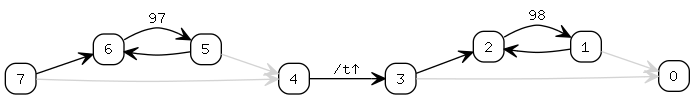
\includegraphics[width=\linewidth]{img/example1/tnfa.png}\\
\footnotesize{TNFA for $a^* 1 b^*$.} \\
\end{center}
\begin{center}
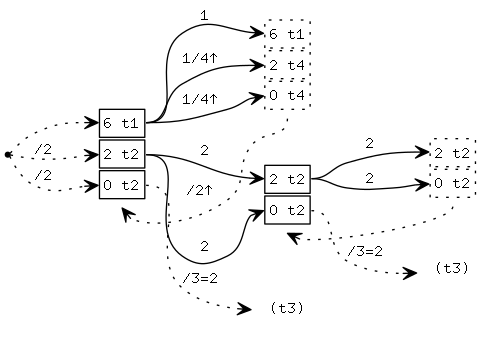
\includegraphics[width=0.8\linewidth]{img/example1/tdfa0_raw.png}\\
\footnotesize{Construction of TDFA(0) for $a^* 1 b^*$.} \\
\end{center}
\begin{center}
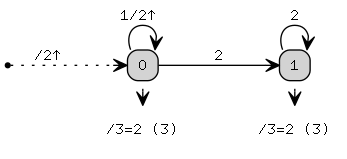
\includegraphics[width=0.6\linewidth]{img/example1/tdfa0.png}\\
\footnotesize{Unoptimized TDFA(0) for $a^* 1 b^*$.} \\
\end{center}
\begin{center}
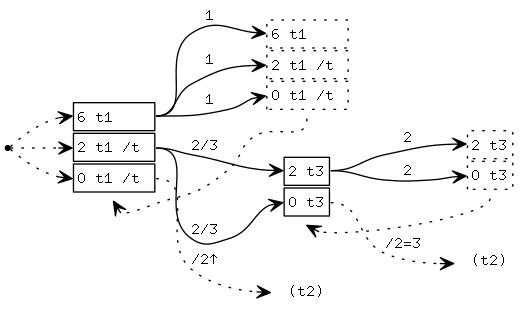
\includegraphics[width=0.8\linewidth]{img/example1/tdfa1_raw.png}\\
\footnotesize{Construction of TDFA(1) for $a^* 1 b^*$.} \\
\end{center}
\begin{center}
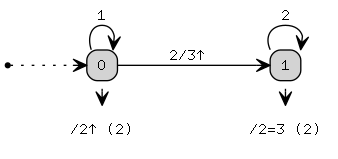
\includegraphics[width=0.6\linewidth]{img/example1/tdfa1.png}\\
\footnotesize{Unoptimized TDFA(1) for $a^* 1 b^*$.} \\
\end{center}

The next example is $a^* 1 a^* a$ --- the same TRE that Lauriakri used to explain his algorithm.
It has a modest degree of nondeterminism: 2 for TDFA(1) and 3 for TDFA(0).
Compare TDFA(0) with figure 3 from [Lau00]: it the same automaton up to a minor notational diffence
(in this case leftmost greedy policy agrees with POSIX).
\begin{center}
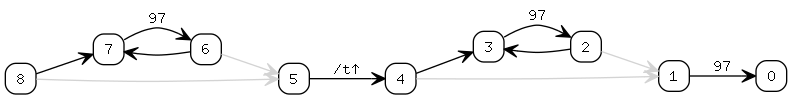
\includegraphics[width=\linewidth]{img/example2/tnfa.png}\\
\footnotesize{TNFA for $a^* 1 a^* a$.} \\
\end{center}
\begin{center}
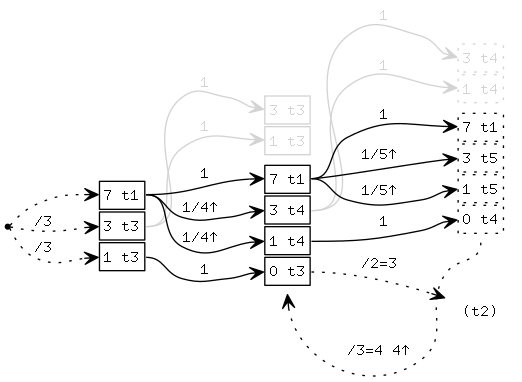
\includegraphics[width=0.8\linewidth]{img/example2/tdfa0_raw.png}\\
\footnotesize{Construction of TDFA(0) for $a^* 1 a^* a$.} \\
\end{center}
\begin{center}
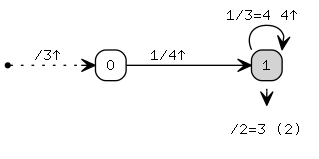
\includegraphics[width=0.6\linewidth]{img/example2/tdfa0.png}\\
\footnotesize{Unoptimized TDFA(0) for $a^* 1 a^* a$.} \\
\end{center}
\begin{center}
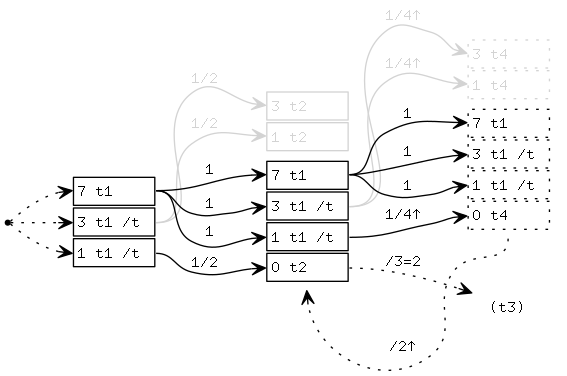
\includegraphics[width=0.8\linewidth]{img/example2/tdfa1_raw.png}\\
\footnotesize{Construction of TDFA(1) for $a^* 1 a^* a$.} \\
\end{center}
\begin{center}
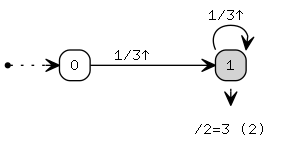
\includegraphics[width=0.5\linewidth]{img/example2/tdfa1.png}\\
\footnotesize{Unoptimized TDFA(1) for $a^* 1 a^* a$.} \\
\end{center}

The next example is $(1 a)^*$.
It shows the typical difference between automata:
TDFA(0) has less states, but more operations; its operations are more clustered and interrelated.
Both automata record the full history of tag on all iterations.
TRE has 2nd degree nondeterminism for TDFA(0) and is deterministic for TDFA(1).
\begin{center}
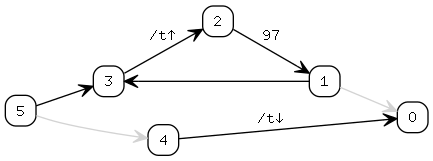
\includegraphics[width=0.6\linewidth]{img/example6/tnfa.png}\\
\footnotesize{TNFA for $(1 a)^*$.} \\
\end{center}
\begin{center}
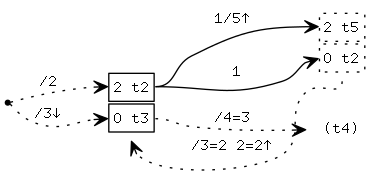
\includegraphics[width=0.6\linewidth]{img/example6/tdfa0_raw.png}\\
\footnotesize{Construction of TDFA(0) for $(1 a)^*$.} \\
\end{center}
\begin{center}
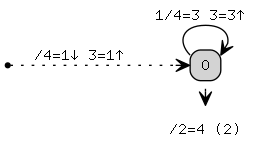
\includegraphics[width=0.5\linewidth]{img/example6/tdfa0.png}\\
\footnotesize{Unoptimized TDFA(0) for $(1 a)^*$.} \\
\end{center}
\begin{center}
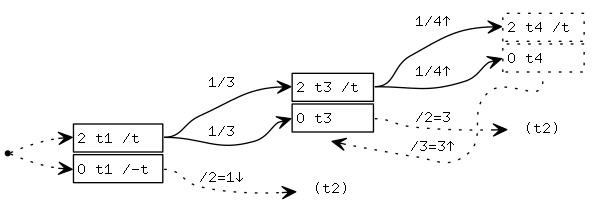
\includegraphics[width=0.9\linewidth]{img/example6/tdfa1_raw.png}\\
\footnotesize{Construction of TDFA(1) for $(1 a)^*$.} \\
\end{center}
\begin{center}
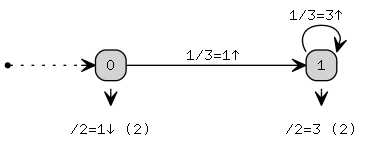
\includegraphics[width=0.6\linewidth]{img/example6/tdfa1.png}\\
\footnotesize{Unoptimized TDFA(1) for $(1 a)^*$.} \\
\end{center}

The next example is $(1 a^+ 2 b^+)^+$.
Like the first example, it shows that TDFA(0) tends to pull operations inside of loops
and behaves much worse than hypothetical hand-written code
(only this example is bigger and gives an idea how the difference between automata changes with TRE size).
If $a^+$ and $b^+$ match multiple iterations (which is likely in practice for TRE of such form), then the difference is considerable.
Both tags have 2nd degree of nondeterminism for TDFA(0), and both are deterministic for TDFA(1).
\begin{center}
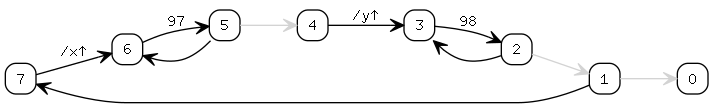
\includegraphics[width=\linewidth]{img/example5/tnfa.png}\\
\footnotesize{TNFA for $(1 a^+ 2 b^+)^+$.} \\
\end{center}
\begin{center}
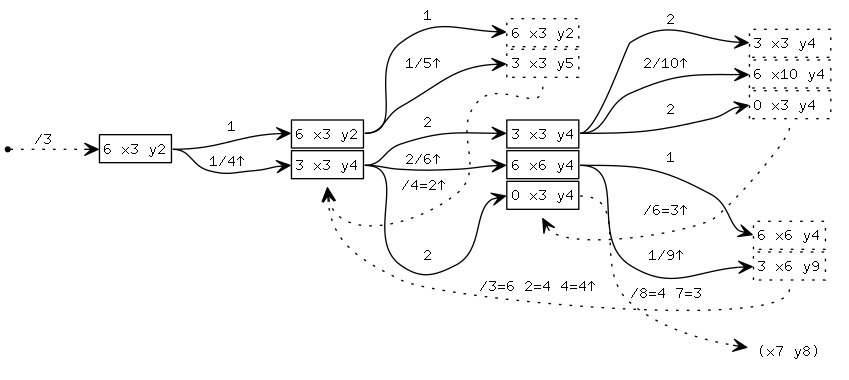
\includegraphics[width=\linewidth]{img/example5/tdfa0_raw.png}\\
\footnotesize{Construction of TDFA(0) for $(1 a^+ 2 b^+)^+$.} \\
\end{center}
\begin{center}
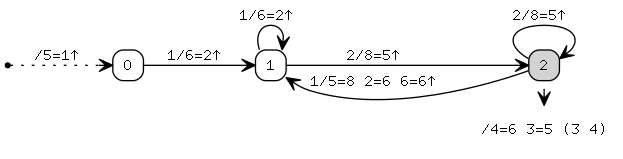
\includegraphics[width=\linewidth]{img/example5/tdfa0.png}\\
\footnotesize{Unoptimized TDFA(0) for $(1 a^+ 2 b^+)^+$.} \\
\end{center}
\begin{center}
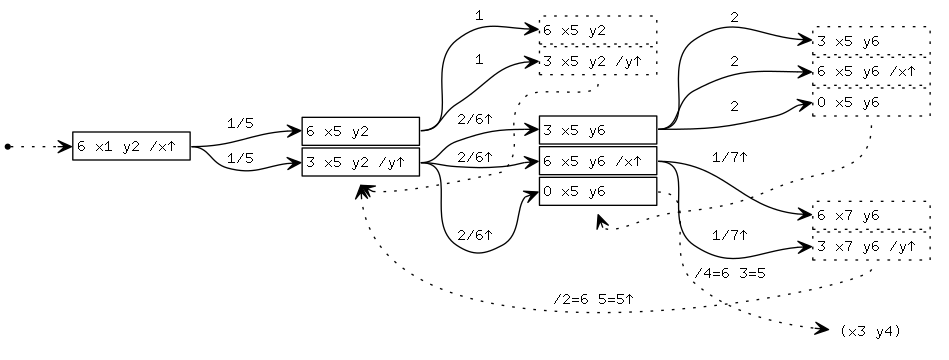
\includegraphics[width=\linewidth]{img/example5/tdfa1_raw.png}\\
\footnotesize{Construction of TDFA(1) for $(1 a^+ 2 b^+)^+$.} \\
\end{center}
\begin{center}
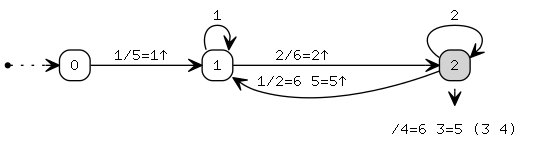
\includegraphics[width=0.8\linewidth]{img/example5/tdfa1.png}\\
\footnotesize{Unoptimized TDFA(1) for $(1 a^+ 2 b^+)^+$.} \\
\end{center}

The next example is $a^* 1 a^{3}$,
which demonstrates a pathological case for both types of automata:
nondeterminism degree grows linearly with the number of repetitions.
As a result, for $n$ repetitions both automata contan $O(n)$ states and $O(n)$ copy operations inside of a loop.
TDFA(0) has one more operation than TDFA(0), but for $n \!>\! 2$ this probably makes little difference.
Obviously, for TRE of such kind both methods are impractical.
However, bounded repetition is a problem on its own, even without tags;
relatively small repetition numbers dramatically increase the size of automaton.
If bounded repetition is necessary, more powerful methods should be used:
e.g. automata with \emph{counters} described in [??].
\begin{center}
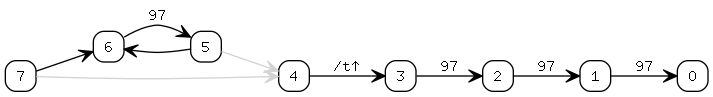
\includegraphics[width=\linewidth]{img/example3/tnfa.png}\\
\footnotesize{TNFA for $a^* 1 a^{3}$.} \\
\end{center}
\begin{center}
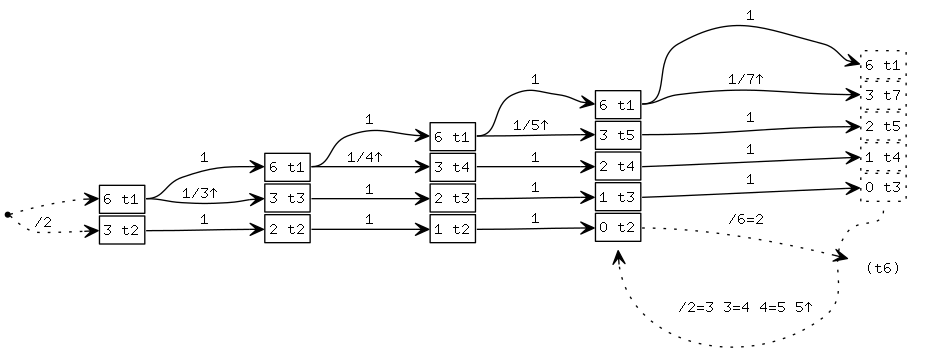
\includegraphics[width=\linewidth]{img/example3/tdfa0_raw.png}\\
\footnotesize{Construction of TDFA(0) for $a^* 1 a^{3}$.} \\
\end{center}
\begin{center}
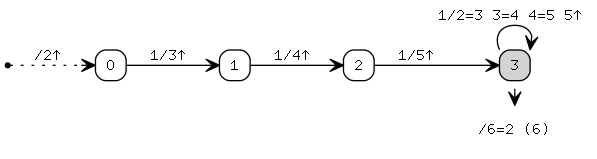
\includegraphics[width=0.8\linewidth]{img/example3/tdfa0.png}\\
\footnotesize{Unoptimized TDFA(0) for $a^* 1 a^{3}$.} \\
\end{center}
\begin{center}
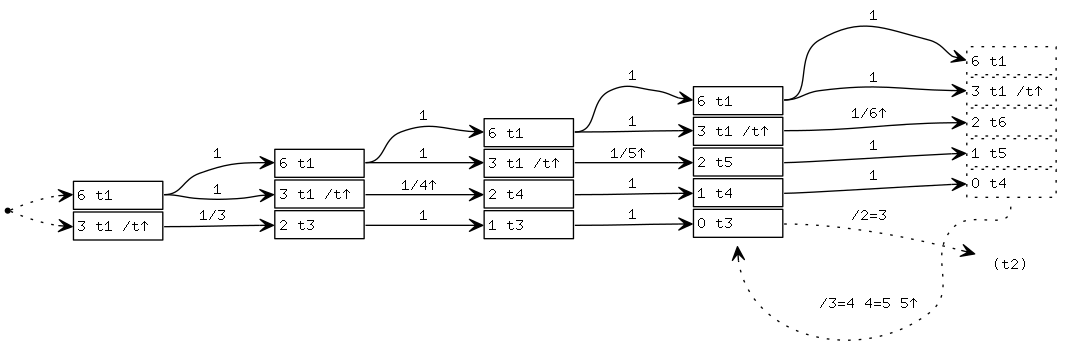
\includegraphics[width=\linewidth]{img/example3/tdfa1_raw.png}\\
\footnotesize{Construction of TDFA(1) for $a^* 1 a^{3}$.} \\
\end{center}
\begin{center}
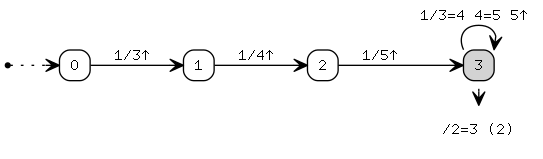
\includegraphics[width=0.8\linewidth]{img/example3/tdfa1.png}\\
\footnotesize{Unoptimized TDFA(1) for $a^* 1 a^{3}$.} \\
\end{center}

Finally, the last example is POSIX RE \texttt{(a|aa)+}, which is represented with TRE $1 (3 (a | aa) 4)^* 2$.
An early optimization in RE2C rewrites it to $1 (3 (a | aa) )^* 4 \, 2$:
orbit tag $4$ is moved out of loop, as we need only its last offset
(disambiguation is based on maximization of tag $3$: as argued in section \ref{section_disambiguation}, checking both tags is redundant).
The resulting automata oscillate between two final states:
submatch result depends on the parity of symbols \texttt{a} in the input string.
Tag $3$ has maximal degree of nondeterminism: $3$ for TDFA(0) and $2$ for TDFA(1).
Tags $2$ and $4$ are deterministic for TDFA(1) and have degree $2$ for TDFA(0).
Tag $1$ is deterministic for both automata.
\begin{center}
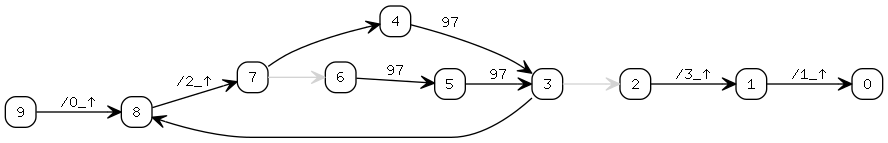
\includegraphics[width=\linewidth]{img/example4/tnfa.png}\\
\footnotesize{TNFA for $1 (3 (a | aa) )^* 4 \, 2$.} \\
\end{center}
\begin{center}
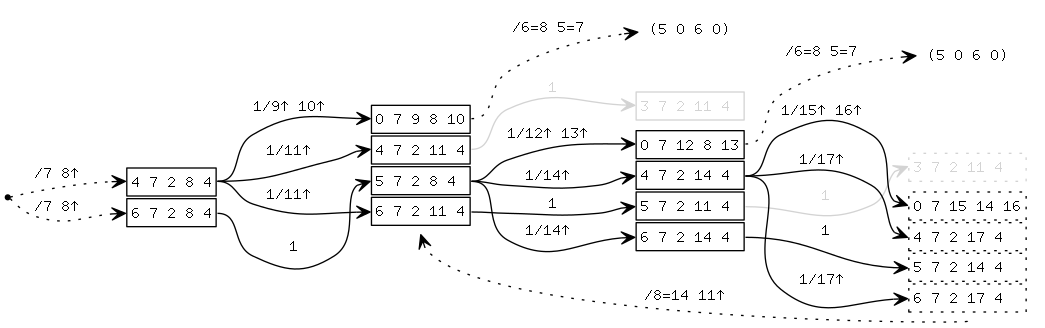
\includegraphics[width=\linewidth]{img/example4/tdfa0_raw.png}\\
\footnotesize{Construction of TDFA(0) for $1 (3 (a | aa) )^* 4 \, 2$.} \\
\end{center}
\begin{center}
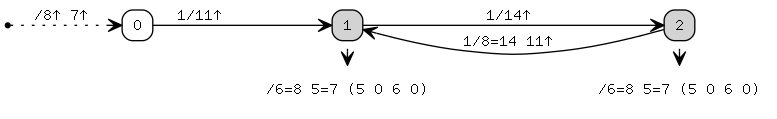
\includegraphics[width=\linewidth]{img/example4/tdfa0.png}\\
\footnotesize{Unoptimized TDFA(0) for $1 (3 (a | aa) )^* 4 \, 2$.} \\
\end{center}
\begin{center}
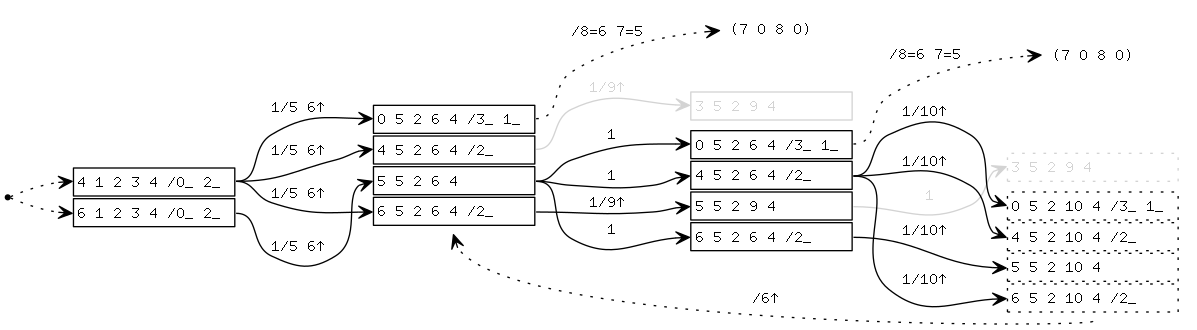
\includegraphics[width=\linewidth]{img/example4/tdfa1_raw.png}\\
\footnotesize{Construction of TDFA(1) for $1 (3 (a | aa) )^* 4 \, 2$.} \\
\end{center}
\begin{center}
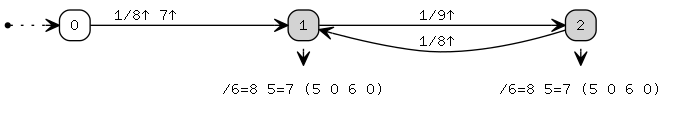
\includegraphics[width=\linewidth]{img/example4/tdfa1.png}\\
\footnotesize{Unoptimized TDFA(1) for $1 (3 (a | aa) )^* 4 \, 2$.} \\
\end{center}

%\vfill\null\pagebreak

%\begin{minipage}{\linewidth}
%    \centering
%    \footnotesize
%    \includegraphics[width=0.5\linewidth]{img/x1.png}
%    \\ A picture of the same gull looking the other way!
%\end{minipage}
%\begin{center}\includegraphics[width=\linewidth]{img/x0.png}\end{center}
%\begin{center}\includegraphics[width=0.5\linewidth]{img/x1.png}\end{center}
%\begin{center}\includegraphics[width=0.5\linewidth]{img/x2.png}\end{center}

\section{Optimizations}\label{section_optimizations}

(1.5x - 2x speedup on in case of RFC-3986 compliant URI parser).

\section{Evaluation}\label{section_evaluation}

\section{Future work}\label{section_future_work}

There is also quite different use of position markers described in literature:
Watson mentions so-called \emph{dotted} RE [Wat95]
that go back to DeRemers's construction of DFA [DeRem74],
which originates in LR parsing invented by Knuth [Knu65]
(\emph{dot} is the well-known LR \emph{item} which separates parsed and unparsed parts of the rule).

\section*{Acknowledgements}

\end{multicols}
\pagebreak

\section*{References}

\begin{enumerate}
\item Laurikari 2000
\item Laurikari 2001
\item Karper
\item Kuklewicz
\end{enumerate}

\end{document}
